% Dokumentenart. Ersetze 12pt, falls die Schriftgröße anzupassen ist.
\documentclass[12pt]{scrartcl}

% Einbinden der Pakete, des Headers und der Formatierung.
% LaTeX Template für Abgaben an der Universität Stuttgart
% Autor: Sandro Speth
% Bei Fragen: Sandro.Speth@studi.informatik.uni-stuttgart.de
%-----------------------------------------------------------
% Modul fuer verwendete Pakete.
% Neue Pakete einfach einfuegen mit dem \usepackage Befehl:
% \usepackage[options]{packagename}
\usepackage[utf8]{inputenc}
\usepackage[T1]{fontenc}
\usepackage[ngerman]{babel}
\usepackage{lmodern}
\usepackage{graphicx}
\usepackage{float}
\usepackage[pdftex,hyperref,dvipsnames]{xcolor}
\usepackage{listings}
\usepackage[a4paper,lmargin={2cm},rmargin={2cm},tmargin={3.5cm},bmargin = {2.5cm},headheight = {4cm}]{geometry}
\usepackage{amsmath,amssymb,amstext,amsthm}
\usepackage[lined,algonl,boxed]{algorithm2e}
\usepackage{algorithmic}
\usepackage{multirow}
% alternative zu algorithm2e:
%\usepackage[]{algorithm} %counter mit chapter
%\usepackage{algpseudocode}
\usepackage{tikz}
\usepackage{hyperref}
\usepackage{url}
\usepackage[inline]{enumitem} % Ermöglicht ändern der enum Item Zahlen
\usepackage[headsepline]{scrlayer-scrpage} 
\usepackage{csquotes}
\pagestyle{scrheadings} 
\usetikzlibrary{automata,positioning,shapes.geometric,trees}

% LaTeX Template für Abgaben an der Universität Stuttgart
% Autor: Sandro Speth
% Bei Fragen: Sandro.Speth@studi.informatik.uni-stuttgart.de
%-----------------------------------------------------------
% Modul beinhaltet Befehl fuer Aufgabennummerierung,
% sowie die Header Informationen.

% Überschreibt enumerate Befehl, sodass 1. Ebene Items mit
\renewcommand{\theenumi}{(\alph{enumi})}
\renewcommand{\theenumii}{(\roman{enumii})}
% (a), (b), etc. nummeriert werden.
\renewcommand{\labelenumi}{\text{\theenumi}}
\renewcommand{\labelenumii}{\text{\theenumii}}

% Counter für das Blatt und die Aufgabennummer.
% Ersetze die Nummer des Übungsblattes und die Nummer der Aufgabe
% den Anforderungen entsprechend.
% Gesetz werden die counter in der hauptdatei, damit siese hier nicht jedes mal verändert werden muss
% Beachte:
% \setcounter{countername}{number}: Legt den Wert des Counters fest
% \stepcounter{countername}: Erhöht den Wert des Counters um 1.
\newcounter{sheetnr}
\newcounter{exnum}

% Befehl für die Aufgabentitel
\newcommand{\exercise}[1]{\section*{Exercise \theexnum\stepcounter{exnum}: #1}} % Befehl für Aufgabentitel

% Formatierung der Kopfzeile
% \ohead: Setzt rechten Teil der Kopfzeile mit
% Namen und Matrikelnummern aller Bearbeiter
\ohead{Hui Zeng}
% \chead{} kann mittleren Kopfzeilen Teil sezten
% \ihead: Setzt linken Teil der Kopfzeile mit
% Modulnamen, Semester und Übungsblattnummer
\ihead{Cloud Computing\\
Summer semester 2021\\
Lecture Notes Summary}

\definecolor{comments}{rgb}{0.41,0.54,0.21}
\definecolor{code}{rgb}{0,0,0}
\definecolor{keyword}{rgb}{0.77,0.48,0.57}
\definecolor{number}{rgb}{0.153,0.5,0}
\definecolor{codeBack}{rgb}{0.85,0.85,0.85}
\definecolor{string}{rgb}{0.81,0.57,0.47}

\lstdefinestyle{stdCode}{
	backgroundcolor=\color{codeBack},   
	commentstyle=\color{comments},
	literate=*{0}{{\textcolor{number}{0}}}{1}%
         {1}{{\textcolor{number}{1}}}{1}%
         {2}{{\textcolor{number}{2}}}{1}%
         {3}{{\textcolor{number}{3}}}{1}%
         {4}{{\textcolor{number}{4}}}{1}%
         {5}{{\textcolor{number}{5}}}{1}%
         {6}{{\textcolor{number}{6}}}{1}%
         {7}{{\textcolor{number}{7}}}{1}%
         {8}{{\textcolor{number}{8}}}{1}%
         {9}{{\textcolor{number}{9}}}{1}%
         {.0}{{\textcolor{number}{.0}}}{1}% Following is to ensure that only periods
         {.1}{{\textcolor{number}{.1}}}{1}% followed by a digit are changed.
         {.2}{{\textcolor{number}{.2}}}{1}%
         {.3}{{\textcolor{number}{.3}}}{1}%
         {.4}{{\textcolor{number}{.4}}}{1}%
         {.5}{{\textcolor{number}{.5}}}{1}%
         {.6}{{\textcolor{number}{.6}}}{1}%
         {.7}{{\textcolor{number}{.7}}}{1}%
         {.8}{{\textcolor{number}{.8}}}{1}%
         {.9}{{\textcolor{number}{.9}}}{1}%
         {\ }{{ }}{1}% handle the space
         ,%
	keywordstyle=\color{keyword},
	numberstyle=\tiny\color{number},
	stringstyle=\color{string},
	basicstyle=\ttfamily\scriptsize,
	breakatwhitespace=false,         
	breaklines=true,                 
	captionpos=b,                    
	keepspaces=true,                 
	numbers=left,                    
	numbersep=5pt,                  
	showspaces=false,                
	showstringspaces=false,
	showtabs=false,                  
	tabsize=2
}

\lstset{
	style=stdCode, language=Java,
  	literate={ö}{{\"o}}1
           {ä}{{\"a}}1
           {ü}{{\"u}}1
}

\tikzset{triangle/.style = {regular polygon, regular polygon sides=3 },
node rotated/.style = {rotate=180},
border rotated/.style = {shape border rotate=180},
astTerminal/.style = {regular polygon, regular polygon sides=3, inner sep=2.5pt, shape border rotate=180},
astLabel/.style = {right=3pt,font=\footnotesize\itshape},
astValue/.style = {below=5pt},
astLine/.style = {edge from parent fork down}
}

\graphicspath{{bilder/}}

\def\ojoin{\setbox0=\hbox{$\bowtie$}%
	\rule[-.02ex]{.25em}{.4pt}\llap{\rule[\ht0]{.25em}{.4pt}}}
\def\leftouterjoin{\mathbin{\ojoin\mkern-5.8mu\bowtie}}
\def\rightouterjoin{\mathbin{\bowtie\mkern-5.8mu\ojoin}}
\def\fullouterjoin{\mathbin{\ojoin\mkern-5.8mu\bowtie\mkern-5.8mu\ojoin}}
% Beginn des eigentlichen Dokuments
\usepackage{color,soul}
\newcommand*\circled[1]{\tikz[baseline=(char.base)]{
		\node[shape=circle,draw,inner sep=2pt] (char) {#1};}}     % number in circles

\begin{document}		
	\pagenumbering{roman}
	\title{Business Analytics}
\author{Hui Zeng \thanks{All notes are summarized from the lecture and tutorial materials provided by Prof. Martin Bichler and his DSS team. Images are retrieved from the lecture as well as tutorial slides.}}
\date{Winter Semester 2020-2021}
\maketitle

\newpage
	\newpage
	\setcounter{tocdepth}{2}
	
	\tableofcontents
	\newpage
	\flushleft
	
	\pagenumbering{arabic}
	\section{Formula Sheet}
\subsection{Basics}
\paragraph{Standard Deviation} $$SD(x) = \sqrt{\frac{1}{n-1}\Sigma_i (x_i - \bar{x})^2}$$
\paragraph{Variance} $$Var(x) = \frac{1}{n-1}\Sigma_i (x_i - \bar{x})^2$$
\paragraph{Covariance} $$Cov(x,y) = \frac{1}{n-1}\Sigma_i (x_i - \bar{x})(y_i - \bar{y})$$
\paragraph{Normal Distribution} $$f(x) = \frac{1}{\sigma \sqrt{2\pi}}e^{-\frac{(x-\mu)^2}{2\sigma^2}}$$
standardized: $$Z = \frac{X - \mu}{\sigma}$$
\paragraph{Probability density function (pdf): f(x)} $$f(x) = P(X = x)$$

\paragraph{Cumulative distribution fuction (cdf): F(x)} $$F(x) = P(X \leq x)$$ $$P(X \geq x) = 1 - F(x)$$  $$P(x_1 \leq X \leq x_2) = F(x_2) - F(x_1)$$
\paragraph{Confidence Interval} $$CI = \left[ \bar{X} - z_{(1 - \frac{\alpha}{2})}\cdot \frac{\sigma}{\sqrt{n}} , \bar{X} + z_{(1 - \frac{\alpha}{2})}\cdot \frac{\sigma}{\sqrt{n}} \right] $$
$$CI = \left[ \bar{X} - t_{(1 - \frac{\alpha}{2})}\cdot \frac{s}{\sqrt{n}} , \bar{X} + t_{(1 - \frac{\alpha}{2})}\cdot \frac{s}{\sqrt{n}} \right] $$
\subsection{Linear Regression}
\subsubsection{First Order Linear Model}

$$Y = \beta_0 + \beta_1 X + \varepsilon$$

\paragraph{OLS Estimator}

\begin{align*}
	\hat{\beta}_1 &= \dfrac{\frac{1}{n-1}\Sigma_i (x_i - \bar{x})(y_i - \bar{y})}{\frac{1}{n-1}\Sigma_i (x_i - \bar{x})^2} = \frac{Cov(x,y)}{Var(x)} \\ \ \\
	\hat{\beta}_0 &= \bar{y} - \hat{\beta}_1\cdot \bar{x} \\ \ \\
	\hat{y} &= \hat{\beta}_0 + \hat{\beta}_1 x
\end{align*}	

\subsubsection{Multiple Linear Regression Model}
$$Y = \beta_0 + \beta_1 X_1 + \beta_2 X_2 + \dots + \beta_k X_k + \varepsilon$$
Formulation in \textbf{matrix form}:
$$\begin{bmatrix}
y_1 \\ y_2 \\ \vdots \\ y_m
\end{bmatrix} = \begin{bmatrix}
1 & X_11 &X_12 &\dots &X_1k \\
1 & X_21 &X_22 &\dots &X_2k \\
\vdots & \vdots &\vdots &\vdots &\vdots \\
1 & X_m1 &X_m2 &\dots &X_mk
\end{bmatrix} \begin{bmatrix}
\beta_0 \\ \beta_1 \\ \beta_2 \\ \vdots \\ \beta_k
\end{bmatrix} + \begin{bmatrix}
\varepsilon_1 \\ \varepsilon_2 \\ \vdots \\ \varepsilon_m
\end{bmatrix}$$
$$[m \times 1] = [m \times (k+1)] \cdot [(k+1) \times 1] + [m \times 1]$$

\paragraph{OLS Estimator} 
\begin{itemize}
	\item Model:
	\begin{align*}
		RSS  &= e^{T} e = (y - X\hat{\beta})^T (y - X\hat{\beta}) \rightarrow \min \\
		\rightarrow  &\frac{\partial RSS}{\partial \beta} = -2X^Ty + 2X^TX\beta= 0
	\end{align*}
	
	\item Solution:
	\begin{align*}
		\hat{\beta} &= (X^TX)^{-1}X^Ty \\ 
		\hat{y} &= X(X^TX)^{-1}X^Ty
	\end{align*}

	


\end{itemize}
\subsubsection{Quality Metrics of Linear Regression Models}
\paragraph{Residual Sum of Squares (RSS)}
An \textbf{unbiased} estimator of RSS of the population is given by 
$$RSS = \Sigma_{i=1}^{n} (y_i - \hat{y}_i)^2$$

\paragraph{Mean Squared Error (MSE)}
$$MSE = \frac{RSS}{N}$$
\paragraph{Root Mean Squared Error (RMSE)}
$$RMSE = \sqrt{MSE}$$
\paragraph{Total Sum of Squares (TSS)} sum of Explained Sum of Squares(ESS) and Residual Sum of Squares(RSS).
\begin{align*}
	\Sigma (y - \bar{y})^2 &= \Sigma (\hat{y} - \bar{y})^2 + \Sigma (y - \hat{y})^2 \\
	TSS &= ESS + RSS
\end{align*}
\paragraph{R-squared $\mathbf{R^2}$} the proportional of explained variablity from the model
$$R^2 = \frac{TSS - RSS}{TSS} = 1 - \frac{RSS}{TSS} = \frac{ESS}{TSS}$$ 


\subsection{Logistic Regression \& Poisson Regression}
\subsubsection{The Logistic Regression Model}
The \textbf{binary} logistic regression model described in \textbf{log odds/logit}:
$$log\_odds  =  \ln(\frac{p(X)}{1 - p(X)}), \quad  \ln(\frac{p(X)}{1 - p(X)}) = \beta_0 + \beta_1 X + \varepsilon$$

The logistic regression model described in \textbf{odds}: 
$$odds = \frac{p(X)}{1 - p(X)}, \quad \frac{p(X)}{1 - p(X)} = e^{\beta_0 + \beta_1 X}$$

\subsubsection{The Logistic Function}
$$Pr[Y|X] = p(X) = \dfrac{e^{\beta_0 + \beta_1 X}}{1 + e^{\beta_0 + \beta_1 X}}$$

\subsubsection{Multiple Logistic Regression Model}
$$\ln(\frac{p(X)}{1 - p(X)}) = \beta_0 + \beta_1 X_1 + \beta_2 X_2 + \dots + \beta_k X_k$$

The logistic function can also be described as a \textbf{sigmoid function} in form $S(x) = \frac{e^x}{1 + e^x} = \sigma(x)$
$$P(X) = \sigma(\beta_0 + \beta_1 X)$$
\subsubsection{The Likelihood Function and Maximum Likelihood Estimator}
\paragraph{likelihood function for Logistic Regression Model}
\begin{align*}
	L &= \Pi_{i=1} p^{y_i}(1-p)^{1-y_i} \\
	&= \Pi_{i=1} \sigma(\beta_0 + \beta_1 X)^{y_i} \cdot (1 - \sigma(\beta_0 + \beta_1 X))^{1-y_i}
\end{align*}
\paragraph{Log of Likelihood Function}
$$LL = \ln(L) = \Sigma_{i=1} ( y_{i} \ln(p) + (1 - y_i)\ln(1-p))$$
\paragraph{Maximum Likelihood Estimator}
\begin{align*}
	\beta = \arg\max_{\beta}(LL) &= \arg\max_{\beta} [\Sigma_{i=1} ( y_{i} \ln(p) + (1 - y_i)\ln(1-p))] \\
	&= \arg\max_{\beta} [\Sigma_{i=1} ( y_{i} \ln(\sigma(\beta_0+\beta_1X)) + (1 - y_i)\ln(1-\sigma(\beta_0 + \beta_1X)))]
\end{align*}

\paragraph{Gradient(partial derivatives) of the LL-Function}: \textbf{chain rule}

with $z = \beta_0+\beta_1X$

$$\frac{\partial LL}{\beta_j} = \Sigma_{i=1} \frac{\partial LL}{\partial p} \cdot \frac{\partial p}{\partial z} \cdot \frac{\partial z}{\partial \beta_j}$$
\begin{align*}
	\frac{\partial LL}{\partial p} &= \frac{y_i}{p} - \frac{1 - y_i}{1 - p} \\
	\frac{\partial p}{\partial z} &= \sigma(z) \cdot(1 - \sigma(z)) \\
	\frac{\partial z}{\partial \beta_0} &= 1 \text{, } \frac{\partial z}{\partial \beta_j} = x_j\\		 
\end{align*}
\begin{align*}
	\frac{\partial LL}{\beta_0} &= \left[ \frac{y_i}{p} - \frac{1 - y_i}{1 - p}\right]  \sigma(z) \cdot(1 - \sigma(z)) = \left[ y_i - \sigma(X\beta) \right] \\
	\frac{\partial LL}{\beta_j} &= \left[ \frac{y_i}{p} - \frac{1 - y_i}{1 - p}\right]  \sigma(z) \cdot(1 - \sigma(z))\cdot x_j = \left[ y_i - \sigma(X\beta) \right] x_j
\end{align*}

\subsubsection{Poisson Regression Model}
$$ln(\mu(x)) = \beta_0 + \beta_1 X_1 + \dots \beta_j X_i$$

\paragraph{random component(dependent variable)}
$$Pr(Y|X) = p(X) = \dfrac{e^{-\mu} \mu^y}{y!} = \dfrac{e^{\beta xy} e^{-e^{\beta x}}}{y!}$$

\paragraph{likelihood function}
$$L(\beta|X,Y) = \Pi_{i=1} p = \Pi_{i=1} \dfrac{e^{\beta x_iy_i} e^{-e^{\beta x}}}{y_i!}$$

\paragraph{The Maximum Likelihood Estimator} 
$$\log L(\beta | X,Y) = \Sigma_{i=1} (\beta x_iy_i - e^{\beta x_i} - \log(y_i!))$$





\subsection{Naive Bayes \& Bayesian Network}
\subsubsection{Bayes Theorem}
\begin{itemize}
	\item single evidence: $$Pr(h|e) = \frac{Pr(h \cap e)}{Pr(e)} = \dfrac{Pr(e|h) \cdot Pr(h)}{Pr(e)}$$
	\item multiple evidence: 
	\begin{align*}
		Pr(h|e_1, e_2, \dots, e_k) &= \dfrac{Pr(e_1 | h) \cdot Pr(e_2 | h) \dots Pr(e_k | h) \cdot Pr(h)}{Pr(e_1, e_2, \dots, e_k)} \\ 
		&= \frac{\Pi_{i=1}^k Pr(e_i|h) \cdot Pr(h)}{Pr(e_1,e_2, \dots e_k)}
	\end{align*}
\end{itemize}

	
\subsubsection{Pr(e)}
\begin{itemize}
	\item If the prior probability $Pr(e_i)$ is \textbf{known}: 
	$$Pr(e_1, e_2, \dots, e_k) = Pr(e_1)\cdot Pr(e_2)\dots Pr(e_k)$$
	\item If the prior probability $Pr(e_i)$ is \textbf{unknown}: law of total probability
	$$Pr(e_1, e_2, \dots, e_k) = Pr(e_1, e_2, \dots, e_k|h)\cdot Pr(h) + Pr(e_1, e_2, \dots, e_k | \neg h) \cdot Pr(\neg h)$$
\end{itemize}

\subsubsection{Chain Rule}
According to the \textbf{directed acyclic graph}, derive the \textbf{joint probability distribution} 

$$Pr(e_1, e_2, \dots, e_k) = \Pi_{i=1} Pr(e_i| e_{i-1}, \dots, e_1) = \Pi_{i=1} Pr(e_i| \text{Parents}(e_i))$$

\subsubsection{Conditional Independence}
\paragraph{conditional independence between hypothesis and evidence} the hypothesis $h$ is only dependent on $e_1, e_2, e_3$, not on $e_4$ (redundant), then 
$$Pr(h | e_1, e_2, e_3, e_4) = Pr(h | e_1, e_2, e_3) $$

\paragraph{conditional independence between hypotheses}

if two hypotheses are \textbf{independent} from each other, then
$$Pr(h_1, h_2 | e_1, e_2) = Pr(h_1|e_1,e_2) \cdot Pr(h_2|e_1,e_2)$$











\subsection{Decision Tree}
\paragraph{Entropy} $\in [0,1]$, measures how much \textbf{additional information required} in \textbf{bits}
	$$\text{entropy}(p_1, \dots, p_n) = - \Sigma_{i=1} ^n p_i \cdot \log_{2} p_i$$
	
\paragraph{Information of Each Attribute Value}
	
	$$\text{info}([c_1, \dots, c_n]) = \text{entropy}(\frac{c_1}{C}, \dots, \frac{c_n}{C})$$ 
	
\paragraph{Information of the Attribute} the \textbf{weighted average} of the \textbf{information needed} from each attribute value. 

Say an attribute has $m$ attribute values/branches,

$$\text{info}([c_1, \dots, c_n]_1, \dots, [c_1, \dots, c_n]_m) = \Sigma_{i=1}^m  \frac{C_m}{N} \cdot \text{info}([c_1, \dots, c_n])_m$$

\paragraph{Information Gain of the Attribute} 

$$\text{Information\_Gain(attribute)} = \text{info(before split by attribute)} - \text{info(after split by attribute)}$$ 

\paragraph{Intrinsic Information of a Attribute} s: size of a leaf from each branch
$$\text{intrinsic\_info}([s_1, \dots, s_n]) = \text{info}([s_1, \dots, s_n])$$

\paragraph{Gain Ratio of a Attribute}

$$\text{Gain\_Ratio(attribute)} = \dfrac{\text{Gain(attribute)}}{\text{Intrinsic\_Info(attribute)}}$$


\subsection{Evaluation}

\paragraph{Accuracy} $$\text{Accuracy} = \frac{TP + TN}{N}$$
\paragraph{Error Rate} $$\text{Error Rate} = 1 - \text{Accuracy} = \frac{FP + FN}{N}$$

\paragraph{True Positive Rate / Recall / Hit Rate} $$\text{True Positive Rate/Recall} = \frac{TP}{TP + FN}$$
\paragraph{True Negative Rate / Specificity} $$\text{True Negative Rate/Specificity} = \frac{TN}{TN + FP}$$
\paragraph{False Positive Rate / False Alarm Rate} $$\text{False Positive Rate/False Alarm Rate} = 1- \text{Specificity} = \frac{FP}{TN + FP}$$

\paragraph{Precision} $$\text{Precision} = \frac{TP}{TP + FP}$$

\subsection{Clustering: Expectation Maximization}
\paragraph{Expectation Step} calculate the probability for \textbf{all instances} in \textbf{each cluster}.
$$Pr(A|x) = \frac{Pr(x|A) \cdot Pr(A)}{Pr(x)} ,\quad Pr(x|A) = \frac{1}{\sqrt{2\pi} \cdot \sigma_A} e^{-\frac{(x - \mu_A)^2}{2\sigma_A^2}}$$
$$Pr(B|x) = \frac{Pr(x|B) \cdot Pr(B)}{Pr(x)} ,\quad Pr(x|B) = \frac{1}{\sqrt{2\pi} \cdot \sigma_B} e^{-\frac{(x - \mu_B)^2}{2\sigma_B^2}}$$

\paragraph{Maximization Step} calculate the weighted mean and weighted variance using \textbf{all instances}. 
$$w_{iA} = Pr(A|x), \quad  w_{iB} = Pr(B|x)$$
$$\mu_A = \frac{w_{1A}x_1 + w_{2A}x_2 + \dots + w_{nA}x_n}{w_{1A} + w_{2A} + \dots + w_{nA}}$$
$$\sigma_A = \sqrt{\frac{w_{1A} (x_1 - \mu_A)^2 + \dots + w_{nA} (x_n - \mu_A)^2}{w_{1A} + w_{2A} + \dots + w_{nA}}}$$
analog to $\mu_B$ and $\sigma_B$

$$Pr(A) = \frac{\Sigma w_A}{\Sigma w_A + \Sigma w_B}, \quad Pr(B) = 1 - Pr(A)$$

\subsection{Principal Component Analysis \& Restoring Original Data}
\begin{figure}[H]
	\centering
	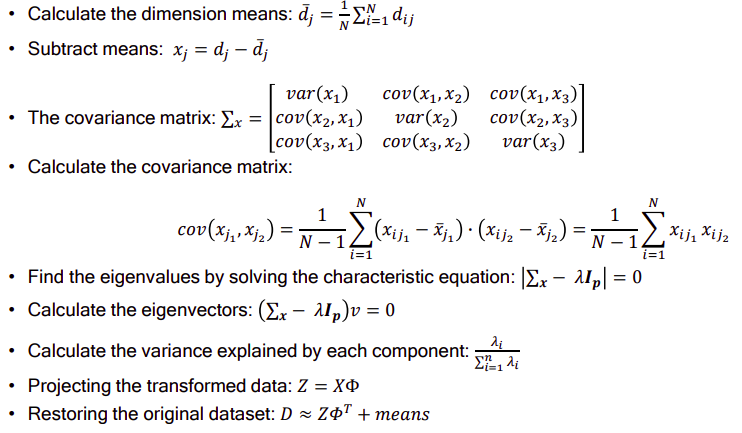
\includegraphics[width=\textwidth]{dimreduce.png}
\end{figure}
\newpage
\subsection{Recommendation Systems: Association Rules}
\paragraph{Support of a Rule}
\item support of \textbf{a rule}: the support of all item sets it contains. 
$$supp(A,B \Rightarrow C,D) = supp(\{A,B,C,D\})$$

\paragraph{Confidence of a Rule}  the probability that X and Y coexist given that X exists.
$$conf(R: X \Rightarrow Y) = \frac{supp(X \cup Y)}{supp(X)}$$

\paragraph{Lift of a Rule} indicates \textbf{by how much (ratio)} the \textbf{confidence of a rule} surpasses the \textbf{expected value}. 
$$Lift(R: X \Rightarrow Y) = \frac{conf(R)}{expConf(R)} = \dfrac{\frac{supp(X \cup Y)}{supp(X)}}{supp(Y)} = \frac{supp(X \cup Y)}{supp(X)\cdot supp(Y)}$$
\subsection{Recommendation Systems: Collaborative Filtering}
\paragraph{Weighted Correlation}
$$w_{a,u} = s_{a,u} \cdot c_{a,u}$$ 
$$c_{a,u} = \frac{Cov(r_{a}, r_{u})}{\sigma_{r_{a}} \cdot \sigma_{r_{u}}}$$
$$Cov(r_{a}, r_{u}) = \frac{1}{m-1}\cdot \Sigma (r_a - \bar{r}_a) (r_u - \bar{r}_u)$$

\paragraph{Rating Prediction}
$$p_{a,i} = \bar{r}_a + \Sigma_{u = 1}^k \dfrac{w_{a,u} \cdot (r_{u,i} - \bar{r}_u)}{\Sigma_{u=1}^k |w_{a,u}|}$$

\subsection{Recommendation Systems: SVD}
\paragraph{Rating Prediction}
$$r_{u,i} = \bar{r}_u + U(user) \cdot S \cdot V^T(item)$$


\subsection{Neural Network}
\paragraph{Forward Pass}
\begin{align*}
	z^{[1]} &= W^{[1]}\cdot a^{[0]} + b^{[1]} =  W^{[1]}\cdot x + b^{[1]}\\
	a^{[1]} &= g^{[1]}(z^{[1]}) = \sigma(z^{[1]}) \\
	z^{[2]} &= W^{[2]}\cdot a^{[1]} + b^{[2]} \\
	a^{[2]} &= g^{[2]}(z^{[2]}) = \sigma(z^{[2]})
\end{align*}

\paragraph{Loss Function} If we evaluate the model using \textbf{cross-entropy loss}: the calculation for $y \ln\hat{y}$ is a dot product(element-wise multiplication).
$$l(y,\hat{y}) = - [y \ln \hat{y} + (1-y)\ln(1 - \hat{y})]$$
\paragraph{Empirical Risk}  \textbf{average} the loss.
$$\mathcal{L}(y,\hat{y}) = \frac{1}{n} \cdot \Sigma l(y,\hat{y})$$

\paragraph{Backpropagation}

example in updating layer 2:
\begin{align*}
	W^{[2]}_{t+1} &= W^{[2]}_t - \alpha \cdot dW =W^{[2]}_t - \alpha \cdot \frac{\partial L}{\partial W^{[2]}} \\
	b^{[2]}_{t+1} &= b^{[2]}_t - \alpha \cdot db =b^{[2]}_t - \alpha \cdot \frac{\partial L}{\partial b^{[2]}} 
\end{align*}

	
$$\frac{\partial L_n}{\partial W} = \frac{\partial L_n}{\partial a_{n}} \cdot \frac{\partial a_{n}}{\partial z_{n}} \cdot \frac{\partial z_n}{\partial W}$$

\begin{align*}
	L_n &= \frac{1}{2} (y_{n} - g(w_{kl}a_{kn} + b_l))^2 = \frac{1}{2} (y_n - a_{ln})^2, \quad &\frac{\partial L_n}{\partial a_{ln}} &= -(y_n - a_{ln})\\
	a_{ln} &= g(z_{ln}) , \quad &\frac{\partial L_n}{\partial z_{ln}} &= g'(z_{ln}) \\
	z_{ln} &= w_{kl}a_{kn} + b_l, \quad &\frac{\partial L_n}{\partial w_{ln}} &= a_{kn} 	
\end{align*}

If the activation is a sigmoid activation: $\sigma(x) = \frac{e^x}{1 + e^x}$, $\sigma'(x) = \sigma(x)(1 - \sigma(x))$.
$$dW^{[2]} = -(y- a^{[2]})\cdot a^{[1]^{T}} = (a^{[2]} - y) \cdot a^{[1]^{T}}$$

\paragraph{Gradient Descent}

	\subparagraph{fixed step size}
	$$\begin{bmatrix}
	x_n \\y_n
	\end{bmatrix} = \begin{bmatrix}
	x_{n-1} \\ y_{n-1}
	\end{bmatrix} - \alpha \cdot \nabla f(x_{n-1}, y_{n-1})$$
	\subparagraph{dynamic step size}
	$$\begin{bmatrix}
	x_n \\y_n
	\end{bmatrix} = \begin{bmatrix}
	x_{n-1} \\ y_{n-1}
	\end{bmatrix} - \alpha_{n} \cdot \nabla f(x_{n-1}, y_{n-1})$$
	
	\subparagraph{Momentum}
	\begin{align*}
		d_n &= \beta \cdot d_{n-1} + \alpha \cdot\nabla f(x_{n-1})\\
		x_n &= x_{n-1} - d_n
	\end{align*}



	\section{Introduction}
Different IT-trends boosts the need for cloud computing:
\begin{itemize}
	\item Outsourcing, either infrastructure or management
	\item IT as a service: pay per use
	\item Re-centralization of data: similar to data centers, cloud be provided as a central place for data storage.
	\item Resource sharing instead of over-provisioning: same resource can be used for multiple purposes
	\item Server consolidation: instead of having multiple physical servers, with each dedicated to a certain service, servers are virtualized and put on one/reduced number of physical machines.     
	\item Scalable computing
	\item Application dynamism: amount of request on web changes over time.
	\item Green computing, big data, stream processing, IoT, machine learning, etc.
\end{itemize}

\paragraph{Cloud Computing} the definition is mainly divided by
\begin{itemize}
	\item ubiquitous, convenient, on-demand network access to a \textbf{shared pool of configurable computing resources} (eg: networks, servers, storage, applications, services)
	\item resources can be \textbf{rapidly provisioned} and released with \textbf{minimal management effort} or service provider interaction
	\item cloud model is composed of 
	\begin{itemize}		
		\item 3 service models
		\item 4 deployment models
		\item 5 essential characteristics
	\end{itemize}
\end{itemize}

\subsection{3 Service Models: IaaS, PaaS and SaaS}
Three service models, ranking from outsourcing the least to the most: IaaS $\rightarrow$ PaaS $\rightarrow$ SaaS.

\subsubsection{IaaS: Infrastructure as a Service}
\begin{itemize}
	\item Offering: provision processing, storage, networks, other fundamental computing resources
	\item Rights as consumer: 
	\begin{itemize}
		\item deploy and run \textbf{arbitrary} software, including \textbf{operating systems and applications}
		\item control over OS, storage, deployed applications
		\item limited control of select networking components
	\end{itemize}
	\item No control as consumer:
	\begin{itemize}
		\item underlying cloud infrastructure
	\end{itemize}
	
	
\end{itemize}
\subsubsection{PaaS: Platform as a Service}
\begin{itemize}
	\item Offering: application infrastructure services(eg: development platforms, libraries, tools, databases) through client interface
	\item Rights as consumer:
	\begin{itemize}
		\item limited user-specific application configuration settings
	\end{itemize}
	\item No control as consumer:
	\begin{itemize}
		\item underlying cloud infrastructure
		\item network, servers, storage, OS
		\item individual application capabilities
	\end{itemize}
	\item Example: MS Azure, Amazon FaaS, Google application engine
\end{itemize}
\subsubsection{SaaS: Software as a Service}
\begin{itemize}
	\item Offering: provider's applications on cloud through client interface
	\item Rights as consumer:
	\begin{itemize}
		\item limited user-specific application configuration settings
	\end{itemize}
	\item No control as consumer:
	\begin{itemize}
		\item underlying cloud infrastructure
		\item network, servers, OS, storage
		\item individual application capabilities
	\end{itemize}
\end{itemize}
\begin{figure}[H]
	\centering
	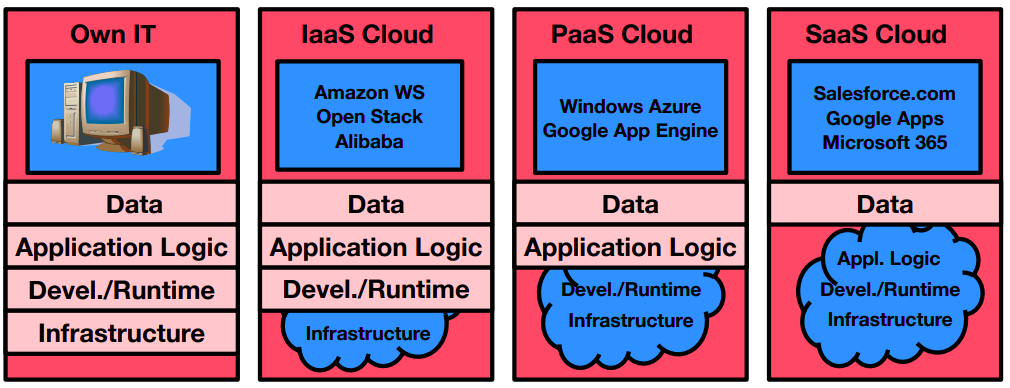
\includegraphics[width=\textwidth]{servicemodels.png}
	%\caption{Comparison over the service models}
\end{figure}
\begin{figure}[H]
	\centering
	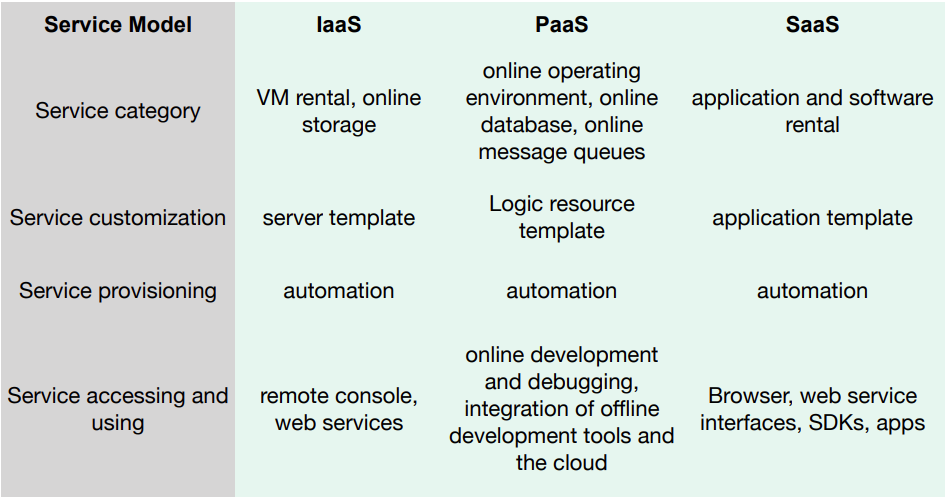
\includegraphics[width=0.8\textwidth]{servicemodel1.png}
	%\caption{Comparison over the service models}
\end{figure}\begin{figure}[H]
\centering
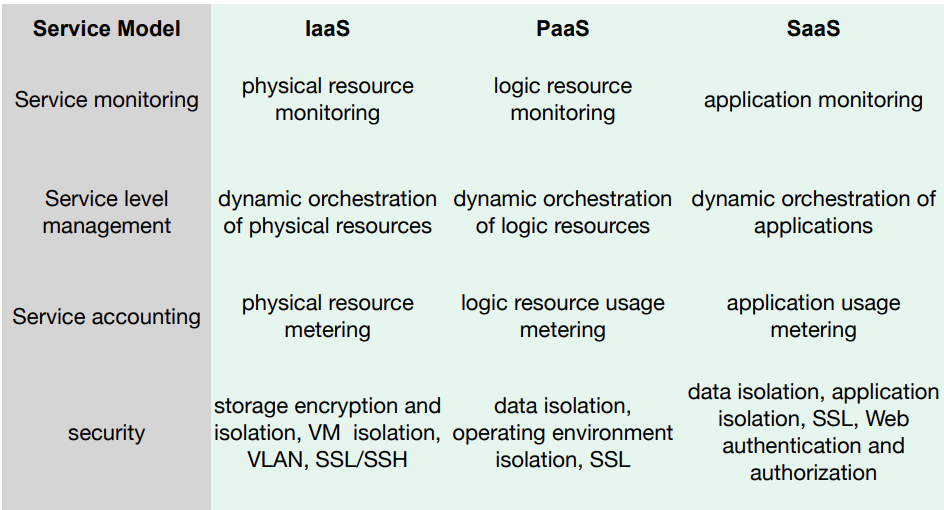
\includegraphics[width=0.8\textwidth]{servicemodel2.png}
%\caption{Comparison over the service models}
\end{figure}
\subsection{4 Deployment Models: Private, Community, Public, Hybrid}
\begin{itemize}
	\item Private Cloud:
	\begin{itemize}
		\item service offered \textbf{via private network} for \textbf{single client}.
	\end{itemize}
	\item Community Cloud:
	\begin{itemize}
		\item service offered to \textbf{a specific group of clients}.
	\end{itemize}
	\item Public Cloud:
	\begin{itemize}
		\item service offered \textbf{over Internet via Web-application} or third-party provider for \textbf{everyone}.
	\end{itemize}
	\item Hybrid Cloud: combination of public and private cloud.
\end{itemize}

\subsection{5 Essential Characteristics}
\begin{itemize}
	\item \textbf{on-demand self-service}: 
	\begin{itemize}
		\item able to \textbf{provision computing capabilities} unilaterally(no interaction required with provider).
	\end{itemize}
	
	\item \textbf{broad network access}: 
	\begin{itemize}
		\item capabilities can be available and accessed through by \textbf{diversely thin or thick client platforms} (mobile, tablets, cable, etc.)
	\end{itemize}
	
	\item \textbf{resource pooling}: 
	\begin{itemize}
		\item \textbf{multi-tenant model} is used, multiple customers shares the computing capabilities at the same time, according to their self-customized demand. Specification of resource location can be possible at higher abstraction level.
	\end{itemize}
	 
	\item \textbf{rapid elasticity}: 
	\begin{itemize}
		\item computing capabilities can be \textbf{elastically provisioned and released} in any quantity at any time. The process can be automated or scaled according to dynamic demand.
	\end{itemize}
	\item \textbf{measured service}: 
	\begin{itemize}
		\item automatically control and optimize resource use by \textbf{leveraging a metering capability}. Resource usage can be monitored, controlled and reported.
	\end{itemize}
\end{itemize}


\subsection{Pros \& Cons of Clouds}
\begin{itemize}
	\item Advantages:

\begin{itemize}
	\item scalability, elasticity
	\item rapid deployment
	\item no capital investment for physical resources
	\item outsourcing of infrastructure management
	\item limited access to on-premise servers
	\item fault tolerance: multiple servers have data replicas, if one node fails, other nodes will replace.
	\item collaboration
\end{itemize}
	\item Disadvantages:
	\begin{itemize}
		\item no control over security, based on ''trust''.
		\item no control over hardware/infrastructure
		\item vendor lockin: service is not standardized, not compatible to other vendors.
		\item cost on monthly fees: if demand for same computational power is constant, fee may be higher than building own hardware. Only recommendable for dynamic demand.
		\item breaking SLAs: your performance may be influenced by other tenants(multi-tenant model).
	\end{itemize}
\end{itemize}
	\newpage
\part{Regression Analysis}
\section{Definition \& Terminology}
Regressions identify \textbf{relationship between dependent and independent variables}.
\begin{itemize}
	\item Association between dependent \& independent variables, 
	\item Impact of independent variables on dependent variables.
	\item Formulation of association/impact in functional form.
	\item Used for 
	\begin{itemize}
		\item descriptive analysis
		\item numerical prediction
		\item time series forcasting
	\end{itemize}
\end{itemize} 
\subsection*{Terminology}
\begin{itemize}
	\item \textbf{measurement tuples}: data streams  $(x_1,y_1), \dots, (x_n,y_n)$
	\item \textbf{predictor (independent variable, feature, regressor, covariate)}: $x_i$
	\item \textbf{response (dependent variable, outcome)}: $y_i$
	\item \textbf{regression function}: $\eta(x) = E(y|x)$
\end{itemize}






\section{Linear Regression}
\subsection{First Order Linear Model}

$$Y = \beta_0 + \beta_1 X + \varepsilon$$

\begin{itemize}
	\item Y: response variable (from measurement tuples)
	\item X: predictor variable (from measurement tuples)
	\item $\beta_0$: y-Axis intercept, \textbf{unknown, to be estimated} 
	\item $\beta_1$: slope, \textbf{unknown, to be estimated}
	\item $\varepsilon$: \textbf{residual}, random error 
\end{itemize}

\subsection{Multiple Linear Regression Model}
$$Y = \beta_0 + \beta_1 X_1 + \beta_2 X_2 + \dots + \beta_k X_k + \varepsilon$$
Formulation in \textbf{matrix form}:
$$\begin{bmatrix}
y_1 \\ y_2 \\ \vdots \\ y_m
\end{bmatrix} = \begin{bmatrix}
1 & X_11 &X_12 &\dots &X_1k \\
1 & X_21 &X_22 &\dots &X_2k \\
\vdots & \vdots &\vdots &\vdots &\vdots \\
1 & X_m1 &X_m2 &\dots &X_mk
\end{bmatrix} \begin{bmatrix}
\beta_0 \\ \beta_1 \\ \beta_2 \\ \vdots \\ \beta_k
\end{bmatrix} + \begin{bmatrix}
\varepsilon_1 \\ \varepsilon_2 \\ \vdots \\ \varepsilon_m
\end{bmatrix}$$
$$[m \times 1] = [m \times (k+1)] \cdot [(k+1) \times 1] + [m \times 1]$$

\textbf{OLS Estimator} for multiple linear regression model: minimize the RSS
\begin{itemize}
	\item Model:
	\begin{align*}
		RSS  &= e^{T} e = (y - X\hat{\beta})^T (y - X\hat{\beta}) \rightarrow \min \\
		\rightarrow  &\frac{\partial RSS}{\partial \beta} = -2X^Ty + 2X^TX\beta= 0
	\end{align*}
	
	\item Solution:
	\begin{align*}
		\hat{\beta} &= (X^TX)^{-1}X^Ty \\ \ \\
		\hat{y} &= X(X^TX)^{-1}X^Ty
	\end{align*}
	
	\item Projection: minimizing RSS $\rightarrow \vec{e}$ is orthogonal to the subspace spanned by all independent variables
	\begin{figure}[H]
		\centering
		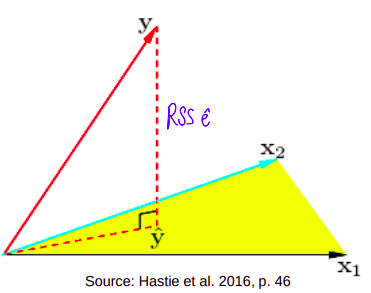
\includegraphics[width=0.4\textwidth]{projection.png}
	\end{figure}
\end{itemize}

\subsection{Estimation of Coefficients: Ordinary Least Square Estimator}
\begin{itemize}
	\item input: data streams $(x_i, y_i)$
		  
		  model: linear regression $Y = \beta_0 + \beta_1 X + \varepsilon$ 
		  
		  output: $\hat{\beta}_0$, $\hat{\beta}_1$
	\item Goal of OLS estimator: \textbf{minimize the sum of squared residuals (RSS) } 
	
	Outlier will have larger value input when residual squared.
	$$\hat{y} = \hat{\beta}_0 + \hat{\beta}_1 x$$
	$$\min{\Sigma_i e_i^2} = \min{\Sigma_i (y - \hat{y})^2} = \min{\Sigma_i (y - (\hat{\beta}_0 + \hat{\beta}_1 x))^2} $$
	
\end{itemize}
\subsection{Quality Metrics of the Model}
To measure how well the model fits the data, you can analyze the quality model-wise or coefficient-wise.
\begin{itemize}
	\item Model-wise: 
	\begin{itemize}
		\item Residual Sum of Squares (RSS)
		\item Total Sum of Squares (TSS)
		\item $R^2$
	\end{itemize}
	\item Coefficient-wise:
	\begin{itemize}
		\item Significance-Test on each coefficient in the model
	\end{itemize}
\end{itemize}
\subsubsection{Residual Sum of Squares (RSS)}
An \textbf{unbiased} estimator of RSS of the population is given by 
$$RSS = \Sigma_{i=1}^{n} (y_i - \hat{y}_i)^2$$
\begin{itemize}
	\item RSS = 0: the model fits 100\% of the data
	\item RSS $\neq$ 0: distance between true $y$ and $\hat{y}$ : residual $e$
	\item RSS $\downarrow$, model-fit quality $\uparrow$
\end{itemize}
\subsubsection{Mean Squared Error (MSE)}
$$MSE = \frac{RSS}{N}$$
\subsubsection{Root Mean Squared Error (RMSE)}
$$RMSE = \sqrt{MSE}$$
\subsubsection{Total Sum of Squares (TSS)}
\textbf{Total Sum of Squares(TSS)} is the sum of Explained Sum of Squares(ESS) and Residual Sum of Squares(RSS).
\begin{align*}
	\Sigma (y - \bar{y})^2 &= \Sigma (\hat{y} - \bar{y})^2 + \Sigma (y - \hat{y})^2 \\
	TSS &= ESS + RSS
\end{align*}
\subsubsection{$\mathbf{R^2}$}
$R^2$ measures the proportion of the variation in y that is explained by the variation in x. $\rightarrow$ the \textbf{proportion of Explained Sum of Squares(ESS).}
$$R^2 = \frac{TSS - RSS}{TSS} = 1 - \frac{RSS}{TSS} = \frac{ESS}{TSS}$$ 
\begin{itemize}
	\item range of $R^2$: [0,1]
	\begin{itemize}
		\item $R^2 = 0$: ESS = 0, RSS = $\infty$. No linear relationship between x and y.
		\item $R^2 = 1$: ESS = TSS, RSS = 0. Perfect match between x and y.
	\end{itemize}
\end{itemize}

\subsubsection{Significance Test of the coefficients: T-Test}
\begin{itemize}
	\item Test the significance of the coefficients in alternative hypothesis($H_1$):
	$$H_0: \beta_1 = 0$$
	$$H_1: \beta_1 \neq 0$$
	\item Distribution: T-Distribution
	\item Degree of Freedom: if \textbf{error variable} is \textbf{normally distributed}, then $$df = n - 2 $$
	\item test statistic:
	\large{$$t = \frac{\hat{\beta}_1 - 0}{SE(\hat{\beta}_1)} = \dfrac{\hat{\beta}_1}{\sqrt{\frac{RSS}{\Sigma_{i=1}^n (x_i - \bar{x})^2} \cdot \frac{1}{n-2}}}$$}
	\item Conclusion: 
	
	two-sided test, reject $H_0$, if $|t| > t^c_{1-\frac{\alpha}{2}}$ or $p < \alpha$
	
\end{itemize}
\subsubsection{Other Metrics}
\begin{itemize}
	\item Adjusted $R^2$: allows models \textbf{with different number of variables} to be compared
	\item F-statistic: indicates linear relationship between y and \textbf{at least one} of the xs
	\item T-test of each partial regression coefficient: significance of a single coefficient while controlling others
\end{itemize}



\subsection{Model Specification}
The process of developing a regression model. It's a repeated process. You need to try different combinations or test the significance of variables to find an optimal regression model.

\begin{itemize}
	\item selection of an appropriate functional form (linear, quadratic, log-linear, interaction terms, etc.)
	\item choosing which variables to include (might include irrelevant or omit relevant variables)
\end{itemize}

\subsubsection{Functional Form of Linear Model} 
\begin{itemize}
	\item standard normal linear model(first-order/multiple)
	\item nominal variables(categorical): 0 or 1
	\item quadratic models: $y = \beta_0 + \beta_1 x_1 + \beta_2 x_2^2 \rightarrow z_2 = x_2^2$ 
	\item interaction terms: $y = \beta_0 + \beta_1 x_1 + \beta_2 x_1x_2 \rightarrow z_2 = x_1x_2$
	\item exponential terms into logarithm terms: $y = \alpha x^{\beta}\varepsilon \rightarrow \ln(y) = \ln(\alpha) + \beta\ln{x} + \ln(\varepsilon)$
\end{itemize}

\subsubsection{Choosing Variables to Include}
\begin{itemize}
	\item Idea: The initial model might include large set of irrelevant variables or omit some relevant variables. 
	\item Goal: find an optimal combination that explains variation in Y with \textbf{a small and meaningful predictors Xs} $\rightarrow$ feature selection
	\item Methods:
	\begin{itemize}
		\item \textbf{Best Subset}: 
		
		Test \textbf{all combinations} ($2^n$) and find out best subset 
		\item \textbf{Backward Elimination}: (top-down)
		
		Start with\textbf{ full model with all variables}, test the significance(t-Test) of the variables.
		
		Consider the predictor with lowest t-statistic/highest p-value: remove the variable if $p > \alpha$ (can't reject $H_0$)  
		\item \textbf{Forward Selection}: (buttom-up)
		
		Start with \textbf{only one variable}, test the significance(t-Test) of the variable.
		
		Only consider the variable with highest t-statistic/lowest p-value: add the variable if $p < \alpha$ (reject $H_0$)
		\item \textbf{Stepwise Regression}: combination of forward/backward selection.
	\end{itemize}
\end{itemize}
 
\subsection{Model Interpretation}
Result of a model fitting can be retrieved by ''summary(model)''
\begin{itemize}
	\item Hypothesis:
	\begin{itemize}
		\item Parameters: 
		
		$H_0$: $\beta_i = 0$
		
		$H_1$: $\beta_i \neq 0$
		\item Whole Model: 
		$H_0$: All predictors are not able to explain the model.
		
		$H_1$: The whole model is statistically significant. 		 
	\end{itemize}
	\item Conclusion: 
	
	for an $\alpha = 0.05$ level, $p > \alpha, \rightarrow$ cannot reject $H_0$, the parameter x is not significant from 0. 
\end{itemize}
\begin{figure}[H]
	\centering
	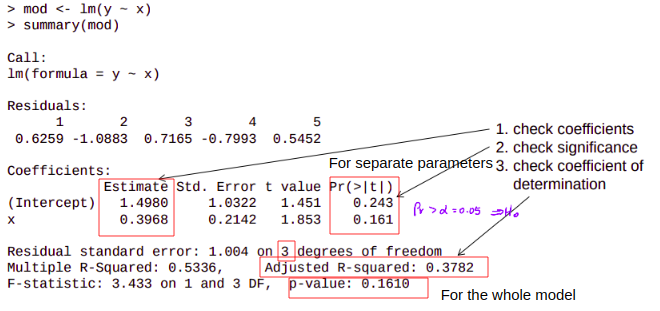
\includegraphics[width=0.9\textwidth]{lm_R.png}
\end{figure}	

\subsubsection*{Interpretation}
\begin{itemize}
	\item \textbf{predictors, intercepts -- coefficient \& p-value}: 
	\begin{itemize}
		\item Significance: significant? at a significance level of $\alpha$ = ?
		\item $\beta_0$: intercept, the value when all predictors are 0.
		\item $\beta_i$: slope, coefficient positive/negative influence of predictors on response? 
		\item \textbf{Transformed} predictors/response
	\end{itemize} 
	\item \textbf{whole model -- F-statistic \& p-value}: significant? at a significance level of $\alpha$ = ?
	\item \textbf{Explanatory power of the model -- Adjusted $R^2$}: high/low? why?
	
\end{itemize}



	\newpage
\part{Regression Diagnostics}
\section{Gauss-Markov Theorem}
The Gauss-Markov theorem states that in a linear regression model, where the errors
\begin{itemize}
	\item have expectation 0
	\item are uncorrelated
	\item have equal variances
\end{itemize}
the \textbf{Best Linear Unbiased Estimator (BLUE)} of the coefficients is given by the \textbf{Ordinary Least Square (OLS)} estimator.
\\ \ \\
Properties of the BLUE:
\begin{itemize}
	\item Unbiased: $E(\hat{\beta}) = \beta$
	\item Consistent: $n \uparrow$, $var(\hat{\beta}) \downarrow$  
	\item Efficient: $var(\hat{\beta}) < var(\tilde{\beta})$, it gives the \textbf{lowest variance} compared to other linear unbiased estimators. 
\end{itemize}

\section{Gauss-Markov Assumptions/Requirements}
The OLS estimator is the best linear unbiased estimator (BLUE), iff
\begin{figure}[H]
	\centering
	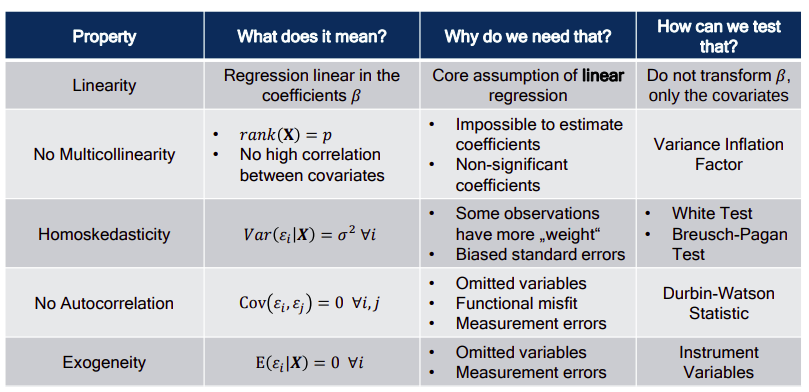
\includegraphics[width=0.9\textwidth]{gauss-markov.png}
\end{figure}
\subsection{Linearity}
\begin{itemize}
	\item Definition: Linear relationship in \textbf{coefficients} $\beta_i$.
	\item Why: core assumption of linear regression.
	\item Solution to non-linearity: Transform the \textbf{predictors or response}(logarithmic, interval-wise)
	\item Influence Factor: \textbf{outliers}. 
	
	Reasons for outlier: 
	\begin{itemize}
		\item error in recording the value
		\item point doesn't belong to the sample
		\item no error, it's an valid observation
	\end{itemize} 
	Solution to outlier:
	\begin{itemize}
		\item identify outliers $\rightarrow$ exclude 
		\item apply ''robust'' regression
	\end{itemize}
\end{itemize}

\subsection{No Multicollinearity}
\begin{itemize}
	\item Definition: \textbf{No} linear dependency between the \textbf{predictors} $X_i$
	
	$\rightarrow$ rank(X) = p (the data matrix has \textbf{full rank} = number of columns)
	
	$\rightarrow$ \textbf{No high correlation} between predictors (though full rank). 
	
	
	
	
	\item Testing: 
	\begin{itemize}
		\item \textbf{Correlation Coefficient} between predictor \textbf{pairs}
		\item \textbf{Variance Inflation Factor (VIF)}: correlation among \textbf{multiple predictors}
		$$VIF = \frac{1}{1-R^2_k}$$
		\paragraph{Interpretation of VIF} 
		
		When the predictor $X_k$ is set as the dependent variable, $R^2_k$ of the variance in the predictor $X_k$ can be explained by the rest of other predictors.
		
		eg: VIF = 10. $R^2_k$ = 90\%. 90\% of the variance in the predictor $X_k$ can be explained by the rest of other predictors.
		
		\paragraph{Rule} VIF $\uparrow$, Multicollinearity $\uparrow$. Remove predictor $X_k$ if $\mathbf{VIF >10}$
		
	\end{itemize}

	\item Consequences of Multicollinearity: Non-significance of the coefficients
	
	The coefficient has a small t-value/large p-value (can't reject $H_0$)
	\begin{itemize}
		\item small VIF: predictor $X_i$ is not related to response 
		
		$\rightarrow$ remove the variable $X_i$
		\item large VIF: predictor $X_i$ is highly correlated to some other predictors. 
		
		$\rightarrow$ \textbf{correlation matrix}: remove one of the highly correlated variables (near 1 or -1)
	\end{itemize}

	\item Example R-Interpretation: 
	\begin{figure}[H]
		\centering
		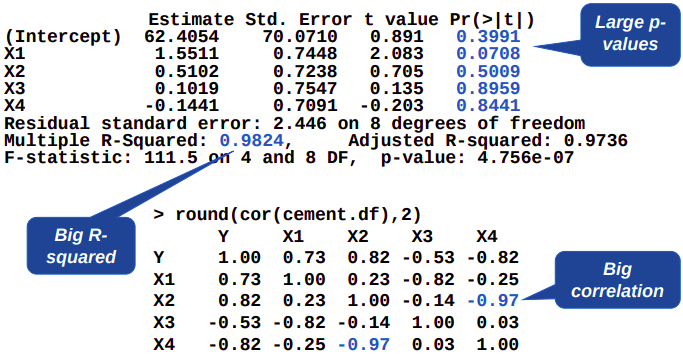
\includegraphics[width=0.6\textwidth]{vif1.png}
	\end{figure}
	\begin{figure}[H]
		\centering
		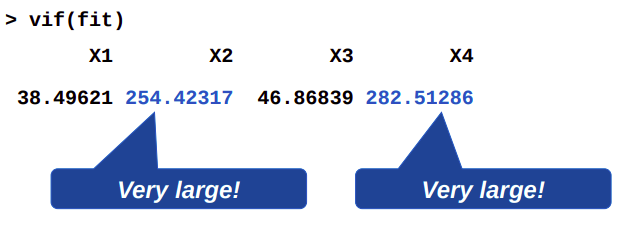
\includegraphics[width=0.6\textwidth]{vif2.png}
	\end{figure}
	large p-value, large VIF $\rightarrow$ high correlation among predictors. Call correlation matrix.
	
	Find out and remove one of the highly correlated predictors.
	\begin{figure}[H]
		\centering
		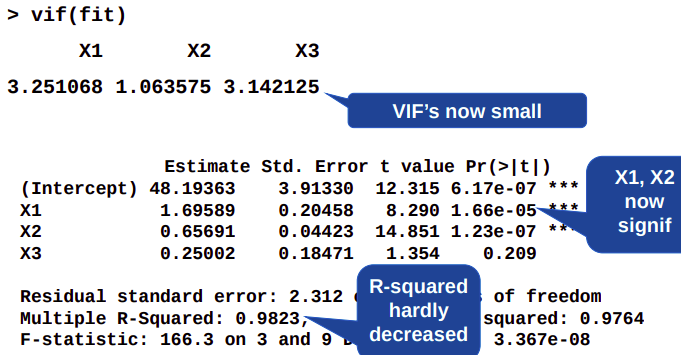
\includegraphics[width=0.6\textwidth]{vif3.png}
	\end{figure}
\end{itemize}

\subsection{Homoscedasticity}
\begin{itemize}
	\item Definition: \textbf{each residual $\sigma_i$} of predictor $X_i$ exhibit \textbf{constant} variance.
	
	$\rightarrow$ the spread of residual in different predictors remains nearly the same. 
	
	$\rightarrow$ no systematic development(grows larger/smaller) of residuals -- \textbf{Heteroscedasticity}
	
	\item Testing: 
	\begin{itemize}
		\item \textbf{Breusch-Pagan Test}
		\item \textbf{White Test}
		\begin{itemize}
			\item $H_0$: all variances $\sigma_i$ are equal (homoscedasticity)
			
			$H_1$: heteroscedasticity
			\item Distribution: $\chi^2$-Distribution
			\item reject $H_0$ if $p < \alpha$ 
		\end{itemize}
	\end{itemize}

	\item Consequence of Heteroscedasticity:
	\begin{itemize}
		\item estimated variance of coefficients $Var(\hat{\beta})$ is \textbf{biased}.
		\item OLS Estimator no longer efficient.
		\item Some predictors has more ''weight'' than others $\rightarrow$ higher sensitivity
	\end{itemize}
\end{itemize}

\subsection{No Autocorrelation}
\begin{itemize}
	\item Definition: no correlation between the $i^{th}$ and $j^{th}$ \textbf{overall residual}
	
	$\rightarrow$ $Cor(\varepsilon_i, \varepsilon_j) = 0$
	
	$\rightarrow$ \textbf{no pattern} of residuals should be observed over time, in case of \textbf{time series data}.
	
	
	\item Testing:
	
	The significance test of coefficients might say they are significant from 0. However, Autocorrelation detected. 
	\begin{itemize}
		\item visualize residuals against time
		\item \textbf{Durbin-Watson statistic [0,4]}: test for first-order autocorrelation
		$$DW = \frac{\Sigma_{i=2}^n (e_i - e_{i-1})^2}{\Sigma_{i=1}^n e_i^2}$$
		\paragraph{Interpretation of DW-statistic}
		\begin{itemize}
			\item DW = 2: \textbf{no} autocorrelation
			
			Rule of thumb: DW $\in$ [1.5, 2.5] $\rightarrow$ no serial correlation
			\item DW = 0: perfect \textbf{positive} autocorrelation
			\item DW = 4: perfect \textbf{negative} autocorrelation
		\end{itemize}
	\end{itemize}

	\item Consequences for autocorrelation:
	\begin{itemize}
		\item an important predictor is omitted (which explains the pattern over time)
		\item functional misfit 
		\item measurement error in predictors
	\end{itemize}

	\item Solution to autocorrelation: Model the missing predictor
	\begin{itemize}
		\item overall trend in time: t 
		\item dummy variable for seasonal indexes $Q_1$, $Q_2$, $Q_3$
		
		number of dummy variables: \textbf{number of choices -1} $\rightarrow$ avoid multicollinearity
	\end{itemize}

	Example Model: 
	$$y = \beta_0 + \beta_1\cdot t + \beta_2 \cdot Q_1 + \beta_3 \cdot Q_2 + \beta_4 \cdot Q_3$$
\end{itemize}

\subsection{Exogeneity}
\begin{itemize}
	\item Definition: the expected value of \textbf{residual vector} given all predictors is 0.
	
	$\rightarrow$ $E(\varepsilon|X) = 0$, $Cov(\varepsilon, X) = 0$
		
	
	\item Consequences for Endogeneity(not exogene):
	\begin{itemize}
		\item measurement error
		\item predictors and response effect each other mutually
		\item \textbf{important predictors are omitted} $\rightarrow$ bias in estimation of coefficients 
	\end{itemize}
	
	\item Testing for individual effects: \textbf{Lagrange Multiplier Test}, in R ''plmtest(model)''
	\begin{itemize}
		\item $H_0$: No individual effects
	\end{itemize}
	\item Testing for fixed or random effect model when Lagrange Multiplier Test fails: \textbf{Hausman Test}
	\begin{itemize}
		\item $H_0$: random effect estimator is consistent \& efficient $\rightarrow$ \textbf{random effect model}
		
		$H_1$: \textbf{fixed effect model} needed.
	\end{itemize}
	
	\item Solution to endogeneity due to omitted variable bias:
	
	according to types of data: 
	\paragraph{cross-section data} data observing many objects at the same time
		
	difficult to find out the confounding variables $\rightarrow$ \textbf{no solution}
	\paragraph{panel data} repeated observations on the same objects over time. Mostly unbalanced panel data, where some individuals are not recorded in all time period. 
	
	$\rightarrow$ individual-specific panel data structure
	
	$\rightarrow$ find out the omitted individual-specific effects on the response.
	
	Solution:
	\begin{itemize}
		\item \textbf{Fixed Effects Model}: 
		Individual/Entity-specific effects are \textbf{correlated} to other predictors
		
		$\rightarrow \lambda_i$ is constant, can be seen as \textbf{an additional intercept} for each individual $i$ in regression model. 
		
		$$y_{it} = (\beta_0 + \lambda_i) + \beta_1 x_{1it} + \beta_2 x_{2it} + \dots + \beta_k x_{kit} + \varepsilon_{it}$$
		
		Estimators for the fixed effect models: first differences, within, least square dummy variable
		\item \textbf{Random Effects Model}: 
		Individual/Entity-specific effects are \textbf{uncorrelated} to other predictors
		
		$\rightarrow \lambda_i$ is drawn independently, can be seen as \textbf{an element of residual} for each individual in regression model.
		$$y_{it} = \beta_0 + \beta_1 x_{1it} + \beta_2 x_{2it} + \dots + \beta_k x_{kit} + \underbrace{(\lambda_i + u_{it})}_{\varepsilon_{it}}$$	
	\end{itemize} 
\end{itemize}



	
\part{Classification Algorithms}
\paragraph{Classification} 
\begin{itemize}
	\item Input: a database $D = {x_1, x_2, \dots, x_n}$ of tuples, a set of classes $C = {C_1, C_2, \dots, C_m}$
	\item Output: a \textbf{mapping} $f: D\rightarrow C$, where each $x_i$ is assigned to a class. 
\end{itemize}
\section{Generalized Linear Models}
\subsection{Component of GLM}
\begin{itemize}
	\item Random component: identifies \textbf{dependent variable $\mu$} and \textbf{its probability function}
	\item Systematc component: identifies the set of \textbf{explanatory variables -- predictors} ($X_1, \dots, X_k$)
	\item Link function: a \textbf{linear} function that links the dependent variable and all explanatory variables.
	$$g(\mu) = \beta_0 + \beta_1 X_1 + \beta_2 X_2 + \dots + \beta_k X_k$$
\end{itemize}
\subsection{Common Link Functions}
\begin{itemize}
	\item \textbf{Identity Link: linear regression}
	$$g(\mu) = \mu = X\beta$$
	\item \textbf{Logit Link: logistic regression}
	$$g(\mu) = \ln(\frac{\mu}{1 - \mu}) = X\beta $$
	\item \textbf{Log Link: Poisson regression}
	$$g(\mu) = \log(\mu) =  X\beta$$
\end{itemize}
\section{Logistic Regression: Binary Classification}
\begin{itemize}
	\item Idea:	
	\begin{itemize}
		\item Gauss-Markov assumptions need to be fulfilled to implement an OLS-Estimator
		
		$\rightarrow$ more \textbf{generalized models} needed to relax the assumptions for OLS
		
		\item Predicting \textbf{categorical dependent variables}: a \textbf{classification} problem.
		\item Limitation from linear regression in classification:
		\begin{itemize}
			\item prediction values $\hat{y}$ should range within [0, 1], linear regression model prediction \textbf{exceeds this range}.
			\item \textbf{violation of Homoscedasticity}: residuals $e_i$ doesn't have constant variance since the true Y only takes two values(0/1). The distribution of the residuals is no longer a normal distribution.
			\item \textbf{violation of No Autocorrelation}: overall residuals of the model follows a systematic pattern, it's positive on one side and negative on the other side $\rightarrow$ Autocorrelation
		\end{itemize}
	\end{itemize}
\end{itemize}

\subsection{The Logistic Regression Model}
The \textbf{binary} logistic regression model described in \textbf{log odds/logit}:
$$\text{log odds} = \ln(\frac{p(X)}{1 - p(X)}) $$
$$\ln(\frac{p(X)}{1 - p(X)}) = \beta_0 + \beta_1 X + \varepsilon$$
\begin{itemize}
	\item Modeling Input: $X_i$, 0/1
	
		  Output: a Logit-model	  
	\item p(X): probability that Y = 1 given X.
	\item \textbf{log odds / logit}: range ($-\infty, +\infty$), the log-ratio of Y = 1 to Y = 0 given X
\end{itemize}

The logistic regression model described in \textbf{odds}: 
$$odds = \frac{p(X)}{1 - p(X)}$$
$$\frac{p(X)}{1 - p(X)} = e^{\beta_0 + \beta_1 X}$$
\begin{itemize}
	\item \textbf{odds}: range [$0, +\infty$), the ratio of Y = 1 to Y = 0 given X
	\begin{itemize}
		\item p(X) = 0.5, odds = 1
		\item p(X) $< 0.5, \rightarrow 0$, odds $\rightarrow 0$
		\item p(X) $> 0.5, \rightarrow 1$, odds $\rightarrow +\infty$
	\end{itemize}
\end{itemize}

\subsection{The Logistic Function}
$$Pr[Y|X] = p(X) = \dfrac{e^{\beta_0 + \beta_1 X}}{1 + e^{\beta_0 + \beta_1 X}}$$
\begin{itemize}
	\item Prediction Input: $X_i$, $\beta_i$
	
	\textbf{Output: $p(X)$}		 
	
	\item Range p(X): [0,1]
	\begin{itemize}
		\item $\beta_0 + \beta_1 X = 0$:  p(X) = 0.5 
		\item $\beta_0 + \beta_1 X  \uparrow$:  p(X) $\rightarrow 1$
		\item $\beta_0 + \beta_1 X  \downarrow$:  p(X) $\rightarrow 0$
	\end{itemize}
	\item $\beta_0$: regression constant, moves the curve \textbf{left/right}
	\item $\beta_1$: regression slope, defines \textbf{steepness} of the curve. $\beta_1 \uparrow$, steepness $\uparrow$
	\item This can be reformed into the logistic regression model. 
	\item Comparison Linear Model \& Logistic Model(the logistic function):
	\begin{figure}[H]
		\centering
		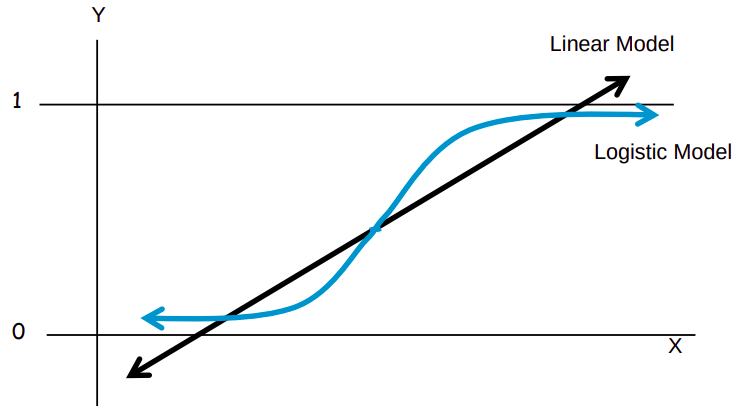
\includegraphics[width=0.6\textwidth]{logit.png}
	\end{figure}
\end{itemize}
Comparison p(X) \& odds \& log-odds:
\begin{figure}[H]
	\centering
	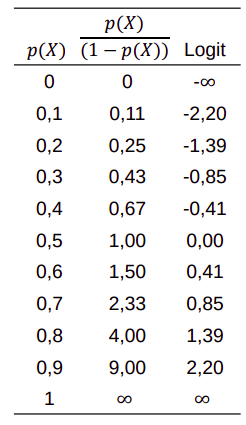
\includegraphics[width=0.25\textwidth]{logodds_odds.png}
\end{figure}

\subsection{Multiple Logistic Regression Model}
$$\ln(\frac{p(X)}{1 - p(X)}) = \beta_0 + \beta_1 X_1 + \beta_2 X_2 + \dots + \beta_k X_k$$
\begin{itemize}
	\item Interpretation of Coefficients $\beta_j$: 
	\begin{itemize}
		\item \textbf{while keeping all other $x_j$ constant}, if $x_{ij}$ increase by 1, the \textbf{log-odds} will increase/decrease by $\beta_j$, or the \textbf{odds} will increase/decrease by $\mathbf{e^{\beta_j}}$.
	\end{itemize}
	\item Test of Multicollinearity: VIF / correlation coefficient
	\item Test of irrelevant variables: Wald-Test (significance of coefficients) 
\end{itemize}

\subsection{Estimation of Coefficients: Maximum Likelihood Estimator}
\subsubsection{Intro}
The probability of one data point $x_i$ can be modeled as \textbf{Bernoulli trial}: 
$$p^{y_i}(1-p)^{1-y_i}$$
The \textbf{likelihood function}:  the \textbf{joint probability} of observing the dependent variable values of random samples. $\rightarrow$ the product of all Bernoulli trials
$$L = \Pi_{i=1} p^{y_i}(1-p)^{1-y_i}$$
The logistic function can also be described as a \textbf{sigmoid function} in form $S(x) = \frac{e^x}{1 + e^x} = \sigma(x)$
$$P(X) = \sigma(\beta_0 + \beta_1 X)$$
\subsubsection{The Likelihood Function and Maximum Likelihood Estimator}
The \textbf{likelihood function for Logistic Regression Model}:
\begin{align*}
	L &= \Pi_{i=1} p^{y_i}(1-p)^{1-y_i} \\
	  &= \Pi_{i=1} \sigma(\beta_0 + \beta_1 X)^{y_i} \cdot (1 - \sigma(\beta_0 + \beta_1 X))^{1-y_i}
\end{align*}

The \textbf{Maximum Likelihood Estimator}: \textbf{maximizes the joint probability} of observing the set of dependent variables of the random samples.
\\ \ \\
Process:
\begin{itemize}
	\item take the log: $$LL = \ln(L) = \Sigma_{i=1} ( y_{i} \ln(p) + (1 - y_i)\ln(1-p))$$
	\item \textbf{maximize} LL: 
	\begin{align*}
		\beta = \arg\max_{\beta}(LL) &= \arg\max_{\beta} [\Sigma_{i=1} ( y_{i} \ln(p) + (1 - y_i)\ln(1-p))] \\
									 &= \arg\max_{\beta} [\Sigma_{i=1} ( y_{i} \ln(\sigma(\beta_0+\beta_1X)) + (1 - y_i)\ln(1-\sigma(\beta_0 + \beta_1X)))]
	\end{align*}
	\item Method: \textbf{Gradient Ascent}
	\begin{figure}[H]
		\centering
		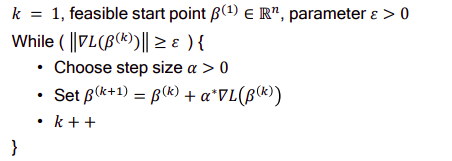
\includegraphics[width=0.65\textwidth]{gradientascent.png}
	\end{figure}
	\begin{itemize}
		\item initial start point
		\item select a step size $\alpha$
		\item compute \textbf{partial derivatives} and \textbf{maximizes the function} $f(x^{(k)} + \alpha \bigtriangledown f(x^{(k)}))$
	\end{itemize}
	\item \textbf{Gradient}(partial derivatives) of the LL-Function: \textbf{chain rule}
	
	 with $z = \beta_0+\beta_1X$
	
	$$\frac{\partial LL}{\beta_j} = \Sigma_{i=1} \frac{\partial LL}{\partial p} \cdot \frac{\partial p}{\partial z} \cdot \frac{\partial z}{\partial \beta_j}$$
	\begin{align*}
		\frac{\partial LL}{\partial p} &= \frac{y_i}{p} - \frac{1 - y_i}{1 - p} \\
		 \frac{\partial p}{\partial z} &= \sigma(z) \cdot(1 - \sigma(z)) \\
		 \frac{\partial z}{\partial \beta_0} &= 1 \text{, } \frac{\partial z}{\partial \beta_j} = x_j\\		 
	\end{align*}
	\begin{align*}
		\frac{\partial LL}{\beta_0} &= \left[ \frac{y_i}{p} - \frac{1 - y_i}{1 - p}\right]  \sigma(z) \cdot(1 - \sigma(z)) = \left[ y_i - \sigma(X\beta) \right] \\
		\frac{\partial LL}{\beta_j} &= \left[ \frac{y_i}{p} - \frac{1 - y_i}{1 - p}\right]  \sigma(z) \cdot(1 - \sigma(z))\cdot x_j = \left[ y_i - \sigma(X\beta) \right] x_j
	\end{align*}
\end{itemize}
\subsection{Quality Metrics of the Model}
\begin{itemize}
	\item \textbf{Null Model}: all predictors $x_i$ has no impact. The model is explained only by the intercept.
	\item \textbf{Fitted Model}: the model is explained by p predictors and 1 intercept.
\end{itemize}

\subsubsection{Null Deviance}
It measures how well the response is explained by \textbf{only the intercept (no predictors)}.
$$\text{null deviance} = -2 \ln(L(null))$$

\subsubsection{Residual Deviance}
$$\text{residual deviance} = -2 \ln(L(fitted))$$
\begin{itemize}
	\item residual deviance $\downarrow$, model quality $\uparrow$
	\item difference between null and residual deviance $\uparrow$, model quality $\uparrow$
\end{itemize}

\subsubsection{AIC}
Additional penalizing term to get a balance between the \textbf{goodness of fit} and \textbf{simplicity of model}.

$$AIC = \text{residual deviance} + 2 \cdot \#\text{parameters in model}$$

\begin{itemize}
	\item AIC $\downarrow$, model quality $\uparrow$
\end{itemize}

\subsubsection{McFadden $\mathbf{R^2}$} the ratio of improvement from null model to fitted model.
$$R_{McFadden}^2 = 1 - \frac{LL(fitted)}{LL(null)} = 1 - \frac{\text{residual deviance}}{\text{null deviance}}$$
\begin{itemize}
	\item model quality $\uparrow$ , LL(fitted) $\ll$ LL(null), $R^2 \rightarrow 1$
	\item model quality $\downarrow$ , LL(fitted) $\approx$ LL(null), $R^2 \rightarrow 0$
	\item rule of thumb: > 0.2 acceptable, > 0.4 ok.
\end{itemize}

\subsubsection{Likelihood Ratio Test}
Does the fitted model explain significantly more variance than null model?
\begin{itemize}
	\item $H_0$: The fitted model explains \textbf{no more variance} than null model
	
	$H_1$: The fitted model explains \textbf{significantly more variance}.
	\item test statistic:
	$$D = -2 \ln (\frac{L(null)}{L(fitted)})$$
	\item Distribution: $\chi^2$-Distribution
\end{itemize}

\subsubsection{Significance Test of Coefficients: Wald Test}
\begin{itemize}
	\item $H_0$: $\beta_i = 0$
	
	$H_1$: $\beta_i \neq 0$
\end{itemize}

\subsubsection{Error Rates}
comparing the predicted classification and the actual classification:
\begin{itemize}
	\item percentage of correct Yes
	\item percentage of correct No
	\item overall percentage of correct predictions
\end{itemize}

\subsection{Model Interpretation}
\subsubsection{R-Result Interpretation}
\begin{figure}[H]
	\centering
	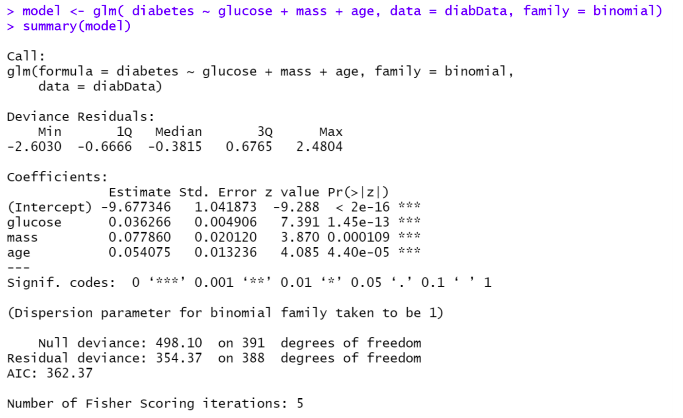
\includegraphics[width=0.75\textwidth]{logit_r.png}
\end{figure}
\begin{itemize}
	\item significance of coefficients: significant if $p < \alpha$ in $\alpha$-level
	\item model: difference between null and residual deviance, AIC
\end{itemize}

\subsubsection{Interpretation of Coefficients}
Effect of change in $x_{ij}$ in \textbf{one unit}:
\begin{figure}[H]
	\centering
	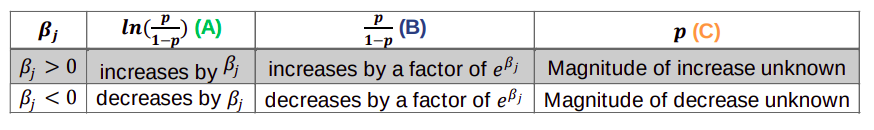
\includegraphics[width=0.9\textwidth]{logit_interpretation.png}
\end{figure}
\begin{itemize}
	\item $\beta_j >0$: 
	\begin{itemize}
		\item If $x_{ij}$ increase by 1, then the \textbf{log odds} will \textbf{increase} by $\beta_j$, or the \textbf{odds} will \textbf{increase} by $\mathbf{e^{\beta_j}}$.
		\item If $x_{ij}$ increase by 1, then the \textbf{log odd ratio} is $\beta_j$, or the \textbf{odd ratio} is $e^{\beta_j}$.
	\end{itemize}
	\item $\beta_j < 0$:
	 \begin{itemize}
	 	\item If $x_{ij}$ increase by 1, then the \textbf{change of log odds} will \textbf{decrease} by $\beta_j$, or the \textbf{change of odds} will \textbf{decrease by a factor} of $\mathbf{e^{\beta_j}}$.
	 	\item If $x_{ij}$ increase by 1, then the \textbf{log odd ratio} is $\beta_j$, or the \textbf{odd ratio} is $e^{\beta_j}$.
	 \end{itemize}
\end{itemize}




\section{Poisson Regression: Binary Classification for Count Data}
\begin{itemize}
	\item Idea: 
	\begin{itemize}
		\item \textbf{count variables (non-negative integers)} as dependent variables
		\item limitation of linear regression / OLS-Estimator
		\begin{itemize}
			\item linear model \textbf{predicts negative values}
			\item count data is often \textbf{highly skewed}: \#crimes committed -- most are 0.
			
			$\rightarrow$ violates normality assumption (residuals follows normal distribution) of OLS-Estimator
		\end{itemize}
	\end{itemize}
	\item Assumption: observed count follows a \textbf{Poisson distribution}.
	$$Pr(y|\mu) = \dfrac{e^{-\mu} \mu^y}{y!}$$
	\begin{itemize}
		\item $\mu$: expected count and expected variance $E(Y) = Var(Y) = \mu$
		\item y: observed count
	\end{itemize} 

	\item Limitation:
	\begin{itemize}
		\item \textbf{Overdispersion}: $E(Y) = Var(Y) = \mu$ not met in real data. 
		
		$\rightarrow$ underestimation of standard errors, potential overconfidence in result. 
		
		$\rightarrow$ Alternative: negative binomial regression
		
		\item \textbf{Zero-inflation}: highly skewed observed data/predictions in 0.
		
		this can't be changed even with negative binomial regression.
	\end{itemize}
	
\end{itemize}
\subsection{Poisson Regression Model}
$$ln(\mu(x)) = \beta_0 + \beta_1 X_1 + \dots \beta_j X_i$$
\subsection{Estimation of Coefficients: Maximum Likelihood Estimator}
The random component(dependent variable) is:
$$Pr(Y|X) = p(X) = \dfrac{e^{-\mu} \mu^y}{y!} = \dfrac{e^{\beta xy} e^{-e^{\beta x}}}{y!}$$

The \textbf{likelihood function}:
$$L(\beta|X,Y) = \Pi_{i=1} p = \Pi_{i=1} \dfrac{e^{\beta x_iy_i} e^{-e^{\beta x}}}{y_i!}$$

The Maximum Likelihood Estimator: 
$$\log L(\beta | X,Y) = \Sigma_{i=1} (\beta x_iy_i - e^{\beta x_i} - \log(y_i!))$$
\begin{itemize}
	\item Method: \textbf{Gradient Ascent}
\end{itemize}
\subsection{Model Interpretation}
R-Result interpretation is same as logistic regression.
\subsubsection{Interpretation of Coefficients}
Effect of change in $X_{ij}$ in \textbf{one unit}:
\begin{figure}[H]
	\centering
	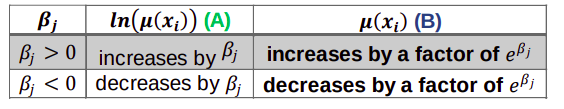
\includegraphics[width=0.65\textwidth]{poisson_coeff.png}
\end{figure}
\begin{itemize}
	\item $\beta_j > 0$: If $x_{ij}$ increases by 1, then the \textbf{log-incidence rate} will \textbf{increase} by $\beta_j$, or the \textbf{incidence rate} will \textbf{increase by a factor} of $e^{\beta_j}$.
	\item $\beta_j < 0$: If $x_{ij}$ increases by 1, then the \textbf{log-incidence rate} will \textbf{decrease} by $\beta_j$, or the \textbf{incidence rate} will \textbf{decrease by a factor} of $e^{\beta_j}$.
\end{itemize}


	\section{Naive Bayes : Multinomial Classification with Independence}
\subsection{Naive Bayes Classifier}
\begin{itemize}
	\item it takes \textbf{all attributes/predictors} into account
	\item Assumptions:
	\begin{itemize}
		\item all attributes are \textbf{equally important}
		\item all attributes are \textbf{independent} $\rightarrow$ no correlation
	\end{itemize}
	\item Difference Regression \& Naive Bayes:
	\begin{itemize}
		\item regression models the importance of different attributes (coefficents $\beta_i$)
		\item attributes from regression can be correlated $\rightarrow$ VIF detection necessary
	\end{itemize}
\end{itemize}

\subsection{Bayes Theorem}
\paragraph{prior / unconditional probability $\mathbf{Pr(e)}$} the probability of a single event $e$
\paragraph{posterior / conditional probability $\mathbf{Pr(e|h)}$} the probability of a single event $e$ given we know $h$
\paragraph{probability distribution $\mathbf{Pr(E)}$} the probability distribution of the random variable $E$, with all possible values $e_i$

\paragraph{Bayes Theorem} 
\subparagraph{single evidence}
\begin{itemize}
	\item Input: 
	\begin{itemize}
		\item $Pr(e)$: prior probability of \textbf{single evidence} $e$ (eg: weather = windy)
		\item $Pr(h)$: prior probability hypothesis (eg: play = true, test = positive)
		\item $Pr(e|h)$: conditional probability of hypothesis 
	\end{itemize} 
	\item Output: posterior conditional probability $Pr(h|e)$
	
	$$Pr(h|e) = \frac{Pr(h \cap e)}{Pr(e)} = \dfrac{Pr(e|h) \cdot Pr(h)}{Pr(e)}$$
or	
	$$Pr(e|h) = \frac{Pr(h \cap e)}{Pr(h)} = \dfrac{Pr(h|e) \cdot Pr(e)}{Pr(h)}$$
	\item If prior probability $Pr(e)$ \textbf{unknown}: law of total probability
	
	$$Pr(e) = Pr(e|h)\cdot Pr(h) + Pr(e|\neg h) \cdot Pr(\neg h)$$
	
	$$Pr(h|e) = \dfrac{Pr(e|h) \cdot Pr(h)}{Pr(e)} = \dfrac{Pr(e|h) \cdot Pr(h)}{Pr(e|h)\cdot Pr(h) + Pr(e|\neg h) \cdot Pr(\neg h)} $$
	
\end{itemize}
\subparagraph{multiple evidences}
\begin{itemize}
	\item Input: 
	\begin{itemize}
		\item $Pr(e_1, e_2, \dots, e_k)$: prior probability of \textbf{multiple evidences} $e_i$
	\end{itemize}
	\item Ouput: posterior conditional probability $Pr(h|e_1, e_2, \dots, e_k)$

	
	$$Pr(h|e_1, e_2, \dots, e_k) = \dfrac{Pr(e_1, e_2, \dots, e_k | h) \cdot Pr(h)}{Pr(e_1, e_2, \dots, e_k)}$$
	Since every attribute/evidence $e_i$ is \textbf{equally important \& independent}:
	\begin{align*}
		Pr(h|e_1, e_2, \dots, e_k) &= \dfrac{Pr(e_1 | h) \cdot Pr(e_2 | h) \dots Pr(e_k | h) \cdot Pr(h)}{Pr(e_1, e_2, \dots, e_k)} \\ 
		&= \frac{\Pi_{i=1}^k Pr(e_i|h) \cdot Pr(h)}{Pr(e_1,e_2, \dots e_k)}
	\end{align*}
	\item If the prior probability $Pr(e_i)$ is \textbf{known}: 
	$$Pr(e_1, e_2, \dots, e_k) = Pr(e_1)\cdot Pr(e_2)\dots Pr(e_k)$$
	\item If the prior probability $Pr(e_i)$ is \textbf{unknown}: law of total probability
	$$Pr(e_1, e_2, \dots, e_k) = Pr(e_1, e_2, \dots, e_k|h)\cdot Pr(h) + Pr(e_1, e_2, \dots, e_k | \neg h) \cdot Pr(\neg h)$$
\end{itemize}



\subsection{Possible Problems in Prediction}

\subsubsection{Zero Frequency Problem in Dataset}
\begin{itemize}
	\item Definition: for the prediction of new instance ,there exists a \textbf{0-frequency} of attribute values \textbf{from the instance attribute}. 
	
	eg: predict whether to play when Outlook = overcast: Pr(Outlook = overcast |$\neg$ play)=0
	
	predict whether to play when Outlook = sunny: \textbf{no} zero-frequency problem here.
	
	\item Solution:
	\begin{itemize}
		\item add 1 to the numerator for \textbf{every attribute value-class combination}.
		
		$\rightarrow$ the prior probability of the result class $Pr(h), Pr(\neg h)$ \textbf{remain the same} though adding 1. 
		
		$\rightarrow$ for small data, significant bias possible
		
		\item assign equal/unequal weights to the numerator, as long as $\Sigma w_i = 1$
	\end{itemize}
\end{itemize}

\subsubsection{Missing Value in New Instance}
\begin{itemize}
	\item Definition: there exists \textbf{missing values} for the attributes in the \textbf{new instance} for prediction.
	\begin{figure}[H]
		\centering
		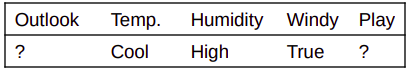
\includegraphics[width=0.45\textwidth]{missingvalue.png}
	\end{figure}
	\item Solution: \textbf{omit} the attribute with missing value in prediction calculation.
	
	$\rightarrow$ take the \textbf{maximum} of $Pr(\text{play} | e_2, e_3,e_4)$ and $Pr(\neg \text{play}|e_2,e_3,e_4)$
\end{itemize}

\subsubsection{Numeric Attributes in Dataset}
\begin{itemize}
	\item Definition: instead of nominal attributes (eg: Outlook = sunny, overcast, cloudy), \textbf{attribute is numeric} (eg: Temperature = 87, 90)
\end{itemize}

\paragraph{Assumption: Attribute Follows Normal Distribution}
\begin{itemize}
	\item Solution:
	\begin{itemize}
		\item Assumption: numeric attributes follows \textbf{normal distribution} $e_i \sim N(\mu,\sigma^2)$
		$$f(x) = \frac{1}{\sqrt{2\pi}\cdot \sigma}\cdot e^{-\frac{(x-\mu)^2}{2 \sigma^2}}$$
		\item calculate the \textbf{mean} and \textbf{standard deviation} for \textbf{each result class}.
		\item conditional probability: \textbf{insert} the numeric instance into the \textbf{probability density function} f(x).
	\end{itemize}
	
	
\end{itemize}

\paragraph{Assumption: Attribute Follows Unknown Distribution}
\begin{itemize}
	\item If the numeric data follows a \textbf{unknown distribution f(x)} (normal distribution not applied) 
	
	$\rightarrow$ probability density distribution \textbf{estimation}.
	\item Solution: kernel density estimation 
	\begin{itemize}
		\item Estimator: Rosenblatt-Parzen Kernel-Density Estimator 
		\item f(x) is not a normal distribution, but each sample follows a normal distribution.
		
		$\rightarrow$ f(x) is the \textbf{sum} of normal distribution at each data point $x_i$
	\end{itemize}
\end{itemize}

\subsection{Prediction using 0-Rule \& 1-Rule}
\begin{itemize}
	\item Input: a dataset $D = x_1, x_2, \dots, x_n$ tuples (evidence, result class), a set of classes $C = C_1, C_2, \dots , C_m$, a \textbf{new instance} with evidence $e_1, \dots, e_k$
	\item Output: classification prediction result 
\end{itemize}
\subsubsection{0-Rule}
Process:
\begin{itemize}
	\item count \textbf{absolute frequency} for each class (classification labels)
	\item Prediction result: class with \textbf{maximum} absolute frequency
\end{itemize}
\subsubsection{1-Rule}
Process:
\begin{itemize}
	\item build \textbf{frequency tables} for each evidence/attribute $e_i$ $\rightarrow$ absolute frequency
	\item pick the \textbf{most frequent class} as classification result for \textbf{each attribute value}
	\item calculate \textbf{overall error rate of the evidence/attribute} according to the classification result
	\begin{figure}[H]
		\centering
		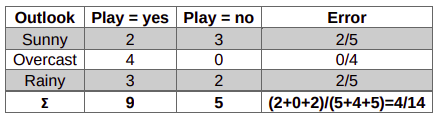
\includegraphics[width=0.45\textwidth]{1-rule.png}
	\end{figure}
	\item Prediction result: choose a \textbf{single attribute} with \textbf{smallest overall error rate}, pick the \textbf{most frequent class} of that evidence/attribute value.
\end{itemize}
Evaluation:
\begin{itemize}
	\item uses only a \textbf{single} attribute for the classification
	\item no prediction result possible if missing value for the attribute found in new instance.
	\item if numeric values in dataset, discretization of the numeric values though possible, but increase the class complexity.
\end{itemize}

\subsection{Prediction using Bayes Theorem: Maximum A Posteriori Classification }
Process:
\begin{itemize}
	\item \textbf{sort} the hypothesis/classification labels, get \textbf{prior probability of hypothesis} $Pr(h), Pr(\neg h)$
	\item  build \textbf{frequency tables} for each evidence/attribute $e_i$ $\rightarrow$ \textbf{absolute frequency}
	\begin{figure}[H]
		\centering
		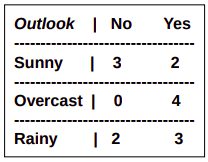
\includegraphics[width=0.25\textwidth]{fre_table.png}
	\end{figure}
	\item check if there is \textbf{zero frequency problem} for the \textbf{attributes from new instance}, resolve by \textbf{adding 1}. 
	
	check for \textbf{numeric} attributes, calculate the \textbf{mean} and \textbf{standard deviation} for each result class.
	\item build \textbf{likelihood tables} for each evidence/attribute $e_i$ $\rightarrow$ \textbf{relative frequency} $Pr(e_i|h)$
	\begin{figure}[H]
		\centering
		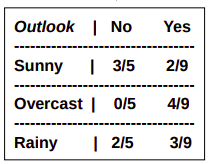
\includegraphics[width=0.25\textwidth]{like_table.png}
	\end{figure}
	\item find $\Pi_{i=1}^k Pr(e_i|h) \cdot Pr(h)$ and $\Pi_{i=1}^k Pr(e_i|\neg h) \cdot Pr(\neg h)$, \textbf{omit} the attribute if \textbf{missing value} in instance.
	\item \textbf{normalize} the result: 
	
	$$Pr(h|e_1,\dots, e_k) = \frac{\Pi_{i=1}^k Pr(e_i|h) \cdot Pr(h)}{Pr(e_1, \dots, e_k)}$$
	$$Pr(\neg h|e_1,\dots, e_k) = \frac{\Pi_{i=1}^k Pr(e_i|\neg h) \cdot Pr(\neg h)}{Pr(e_1, \dots, e_k)}$$ 
	with
	$$Pr(e_1, \dots, e_k) = \Pi_{i=1}^k Pr(e_i|h) \cdot Pr(h) + \Pi_{i=1}^k Pr(e_i|\neg h) \cdot Pr(\neg h)$$

	\item Prediction result: take the \textbf{maximum}.
	$$\text{result} = \max\left\lbrace Pr(h|e_1,\dots, e_k), Pr(\neg h|e_1,\dots, e_k)\right\rbrace $$
\end{itemize}



\subsection{Evaluation of Naive Bayes}
\begin{itemize}
	\item Complexity: 
	\begin{itemize}
		\item calculation of conditional probability: $\mathcal{O}(n)$, 
		
		n: number of instances
		\item calculation of class: $\mathcal{O}(c\cdot p)$, 
		
		c: number of classes, p: number of attributes
	\end{itemize}
	
	\item Advantages: 
	\begin{itemize}
		\item multinomial classification
		\item works well, even if independence assumption is sometimes violated.
	\end{itemize}
	\item Disadvantages:
	\begin{itemize}
		\item takes all attributes with equal weight, could be \textbf{redundant}.
		\item many numeric attributes are actually \textbf{not normally distributed}. 
	\end{itemize}
\end{itemize}

\section{Bayesian Network: Multinomial Classification with Denpendency}

\begin{itemize}
	\item Idea: 
	\begin{itemize}
		\item Naive Bayes assumption too restrictive: \textbf{all} attributes are conditionally independent and equally important.
		\item Attributes are often \textbf{correlated/dependent with each other}
		\item Some attributes are \textbf{redundant} to the classification result.
	\end{itemize}	
	$\rightarrow$ conditional independence among \textbf{subset} of attributes.
\end{itemize}

\subsection{Representation of Bayesian Network: Directed Acyclic Graph}
\begin{itemize}
		\item nodes: attributes
		\item edges: end node is dependent on start node / start node has direct influence on end node.
		\begin{itemize}
			\item start: trigger/cause, evidence node
			\item end: result/effect. 
		\end{itemize}
	\end{itemize}

\begin{figure}[H]
	\centering
	\begin{minipage}{0.5\textwidth}
		\centering
		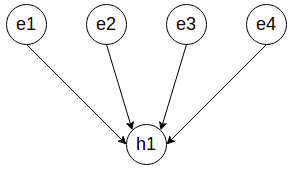
\includegraphics[width=0.45\linewidth]{dag_naivebayes.png}
	\end{minipage}%
	\begin{minipage}{.5\textwidth}
		\centering
		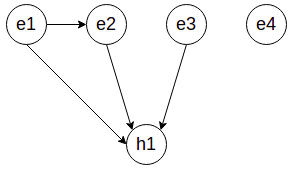
\includegraphics[width=0.45\linewidth]{dag_bayesnet.png}
	\end{minipage}
	\caption{DAG - Naive Bayes(left) vs. Bayesian Network(right)}
\end{figure}
\subsection{Probability Law in Bayesian Network}
\subsubsection{Chain Rule}
According to the \textbf{directed acyclic graph}, derive the \textbf{joint probability distribution} 
	
	$$Pr(e_1, e_2, \dots, e_k) = \Pi_{i=1} Pr(e_i| e_{i-1}, \dots, e_1) = \Pi_{i=1} Pr(e_i| \text{Parents}(e_i))$$
\\ \ \\	
eg: $Pr(A,B,C,D,E) = Pr(A)\cdot Pr(B) \cdot Pr(C|A,B) \cdot Pr(D|A,B,C) \cdot Pr(E|A,C,D)$


\subsubsection{Conditional Independence}
\paragraph{conditional independence between hypothesis and evidence} the hypothesis $h$ is only dependent on $e_1, e_2, e_3$, not on $e_4$ (redundant), then 
	 $$Pr(h | e_1, e_2, e_3, e_4) = Pr(h | e_1, e_2, e_3) $$

\paragraph{conditional independence between hypotheses}

 if two hypotheses are \textbf{independent} from each other, then
	$$Pr(h_1, h_2 | e_1, e_2) = Pr(h_1|e_1,e_2) \cdot Pr(h_2|e_1,e_2)$$

\subsection{Inference in Bayesian Networks}
\begin{itemize}
	\item Idea: infer the probability of an event, given only observation of \textbf{a subset} of other attributes. 
	
	$\rightarrow$ explain the \textbf{away effect} of attributes.
	\item Inference Rules: using \textbf{d-separation}
	\begin{figure}[H]
		\centering
		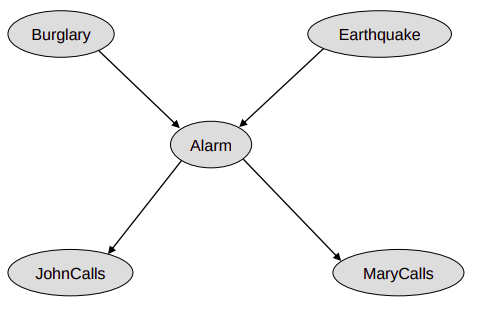
\includegraphics[width=0.4\textwidth]{baynet_example.png}
	\end{figure}
	Example:
	\begin{itemize}
		\item alarm \textbf{not observed}: Burglary \& Mary-calls \textbf{dependent}
				
		$\rightarrow$ if B, belief M $\uparrow$. if M, belief B $\uparrow$.
		
		\item alarm \textbf{observed}: Burglary \& Mary-calls \textbf{conditionally independent}.
				
		$\rightarrow$ no alarm. if Mary-calls, belief B $-$. if B, belief M $-$. 
	\end{itemize}
\end{itemize}

\subsection{Evaluation of a Bayesian Network}
\begin{itemize}
	\item Quality Metrics:
	\begin{itemize}
		\item To maximize the joint probability of training data, the Log-Likelihood of the training data.
		\item Akaike Information Criterion (AIC)
	\end{itemize}
	\item Advantages:
	\begin{itemize}
		\item can handle dependencies among the attributes
	\end{itemize}
	\item Disadvantages:
	\begin{itemize}
		\item computationally expensive, given whether the network structure (DAG) is given, whether the attributes are observable.
	\end{itemize}
\end{itemize}

	\section{Decision Tree Classifiers}
\begin{itemize}
	\item Idea of a Tree: 
	\begin{itemize}
		\item easy to read \& interpret
		\item robust, though lack of solid theoretical/statistical foundations
		\item can use with Ensemble-Methods
	\end{itemize}
\end{itemize}

\subsection{Setup of a Decision Tree}
\begin{itemize}
	\item internal node: test on a \textbf{attribute}
	\item branch: outcome of the test (eg: true/false, red/green)
	\item leaf node: the \textbf{classification label/result}
\end{itemize}

Building an \textbf{Optimal} Decision Tree:
\begin{itemize}
	\item Search Space: $2^{2^m}$ possible trees (m: \# attributes, 2 result classes)
	\item Complexity: \textbf{NP-complete}
	\item Solution: \textbf{Greedy Algorithm} in \textbf{top-down} approach
	\begin{itemize}
		\item All training data at the \textbf{root}.
		\item Partition data \textbf{recursively} by choosing \textbf{one attribute} at each level.
		\item Each split is assessed with a \textbf{measure}
		\item Attribute with \textbf{best split} is chosen.
		\item Repeat until all \textbf{leaf nodes} are pure (Not all attributes are necessary).
	\end{itemize}
\end{itemize}

\subsection{Quality Metrics of a Splitting Attribute}
\begin{itemize}
	\item Idea: 
	\begin{itemize}
		\item the path to classification \textbf{as easy as possible}. $\rightarrow$ \textbf{smallest} tree
		\item good separation of classes $\rightarrow$ leaf nodes gives \textbf{one single class} $\rightarrow$ direct decision
		\item the separation shouldn't affect class distribution.
	\end{itemize}
	\item Evaluation function:
	\begin{itemize}
		\item \textbf{information gain (ID3/C4.5)}
		\item \textbf{information gain ratio}
		\item \textbf{gini index (CART)}
	\end{itemize}
\end{itemize}

\subsubsection{Information Gain}
\begin{itemize}
	\item Idea: choose the attribute that result in \textbf{smallest tree} $\rightarrow$ \textbf{purest} nodes (one class)
	
	$\rightarrow$ choose the attribute with \textbf{greatest information gain}
	
	$\rightarrow$ information gain $\uparrow$, subset average purity $\uparrow$
	
	
	\item Parameters:
	\begin{itemize}
		\item $c_i$: the \textbf{absolute frequency} of the training examples in the class $i$
		\item $C$: the \textbf{total number} of training example at the \textbf{current stage/attribute value}.
		\item $p_i$: the \textbf{relative frequency} of class $i$, $$p_i = \frac{c_i}{C}$$
		\item $N$: the \textbf{total number of training data}
	\end{itemize}
\end{itemize}

\paragraph{Process: }
\begin{enumerate} [label= \protect \circled{\arabic*} ]
	\item calculate \textbf{initial information} before any splits.
	\item calculate \textbf{information for each attribute value} using entropy
	\paragraph{Entropy} $\in [0,1]$, measures how much \textbf{additional information required} in \textbf{bits}
	$$\text{entropy}(p_1, \dots, p_n) = - \Sigma_{i=1} ^n p_i \cdot \log_{2} p_i$$
	\begin{itemize}
		\item entropy = 0: pure
		\item entropy = 1: maximum impurity (for boolean)
	\end{itemize}
	\paragraph{Information of Each Attribute Value} 
	
	$$\text{info}([c_1, \dots, c_n]) = \text{entropy}(\frac{c_1}{C}, \dots, \frac{c_n}{C})$$ 
	\item calculate \textbf{information of the attribute} 
	\paragraph{Information of the Attribute} the \textbf{weighted average} of the \textbf{information needed} from each attribute value. 
	
	Say an attribute has $m$ attribute values/branches,
	
	$$\text{info}([c_1, \dots, c_n]_1, \dots, [c_1, \dots, c_n]_m) = \Sigma_{i=1}^m  \frac{C_m}{N} \cdot \text{info}([c_1, \dots, c_n])_m$$
	
	
	\item calculate the \textbf{information gain}	
	
	\paragraph{Information Gain of the Attribute} 
	
	$$\text{Information\_Gain(attribute)} = \text{info(before split by attribute)} - \text{info(after split by attribute)}$$ 
	
	\item choose the attribute with \textbf{maximum} information gain. 
	\item continue to split. 
	
	\textbf{Attention}: the info \textbf{before} the split is the \textbf{info(attribute value)}, the information gain of the attribute changes to 
	
	eg: gain(Temperature) = \textbf{info(Outlook = sunny)} - info(high, mild, cool)
\end{enumerate}

\paragraph{Limitations}
\begin{itemize}
	\item \textbf{biased} against \textbf{highly-branching} attributes (eg: IDs)
	
	$\rightarrow$ overfitting
	
	$\rightarrow$ Alternative: \textbf{Gain Ratio}
\end{itemize}

\subsubsection{Gain Ratio}
\begin{itemize}
	\item Idea: modification of information gain, reduce bias on highly-branching attributes.
	
	$\rightarrow$ considers \textbf{number and size} of branches $\rightarrow$ \textbf{intrinsic information} of attribute
	
	\item \textbf{Intrinsic Information}, s: size of a leaf from each branch
	$$\text{intrinsic\_info}([s_1, \dots, s_n]) = \text{info}([s_1, \dots, s_n])$$
	eg: 14 IDs, intrinsic\_info([1,1,...,1]) = info([1,1,...,1]) = $14 \cdot (-\frac{1}{14} \cdot \log_{2} \frac{1}{14}) = 3.807$ bits 
	
	\item \textbf{Gain Ratio}: 
	
	$$\text{Gain\_Ratio(attribute)} = \dfrac{\text{Gain(attribute)}}{\text{Intrinsic\_Info(attribute)}}$$
	
	\item Process:
	\begin{itemize}
		\item calculate the \textbf{information gain} of the attribute
		\item calculate the \textbf{intrinsic information} of the attribute
		\item calculate the \textbf{gain ratio}
		\item choose the attribute that has \textbf{maximium} the gain ratio.
	\end{itemize}
\end{itemize}

\subsubsection{Gini Index}
\begin{itemize}
	\item Use-case: in Classification and Regression Tree (CART)
	\item Solution: select the split that \textbf{decreases} the Gini Index \textbf{the most}.
	\item \textbf{Gini Index}: 
	$$Gini(S) = 1 - P^2 - N^2$$
	$$P = \frac{p}{p+n}, N = \frac{n}{p+n}$$
	\item a dataset S is split into $S_1, S_2$, 
	$$Gini_{split} (S_1,S_2) = \frac{p_1 + n_1}{p+n} \cdot Gini(S_1) + \frac{p_2 + n_2}{p+n} \cdot Gini(S_2)$$
	
	$\rightarrow$ select the attribute with \textbf{lowest} Gini-Index after split.
\end{itemize}

\subsection{Evaluation of Decision Tree Algorithm}
\begin{itemize}
	\item Time Complexity: $\mathcal{O}(m\cdot n \log n)$
	
	(m: \# attributes, n: \# instances)
	\item Scalability for large data:
	\begin{itemize}
		\item number of attributes $\uparrow$, tree size $\uparrow$, computation time $\uparrow$.
		\item number of data instances $\uparrow$, memory $\uparrow$
	\end{itemize} 
\end{itemize}

\subsection{Possible Problems in Prediction}
\subsubsection{Numeric Attributes in Dataset}
\begin{itemize}
	\item Solution: \textbf{binary split}
	\item Process:
	\begin{itemize}
		\item an \textbf{initial split point} is either given or the middle of the sorted numeric values.
		\item values are separated into 2 sections: \textbf{below(<)} and \textbf{above($\geq$)} the split point.
		\item calculate \textbf{information gain}
		\item repeat \textbf{binary split}, choose the split with \textbf{maiximum information gain}. 
	\end{itemize}
\end{itemize}

\subsubsection{Missing Values in Dataset}
\begin{itemize}
	\item Possible solutions:
	\begin{itemize}
		\item \textbf{ignore} the instance/attribute with missing values.
		\item treat missing value as \textbf{another nominal value}.
		\item \textbf{estimate} missing values (regression, imputation)
		\item \textbf{follow the leader}: if an instance has missing attribute value, follow the the \textbf{branch with most instances}.
		\item \textbf{partition} the instance: send down instance \textbf{proportionally} to the number of instances. 
		
		$\rightarrow$ classification result is \textbf{weighted}.
	\end{itemize}
\end{itemize}

\subsubsection{Overfitting of the Decision Tree}
\begin{itemize}
	\item Consequences in Overfitting:
	\begin{itemize}
		\item decision tree to \textbf{large \& complex}
		\item \textbf{low bias} on training set, \textbf{high variance} on test set.
		\item poor generalization to new data.
	\end{itemize}
	\item Solution: Pruning 
\end{itemize}

\subsection{Pruning of Decision Trees}
\subsubsection{Prepruning}
Process:
\begin{itemize}
	\item define a \textbf{threshold} when to stop creating subtrees. This should be the same measure as determining attributes (eg: information gain)
	\item \textbf{stop} if the measure \textbf{no longer exceeds threshold}. (eg: infomation gain)
	\item leaf node: the \textbf{most frequent class}
\end{itemize}
Difficult to achieve high performance in practice.

\subsubsection{Postpruning}
\begin{itemize}
	
	\item Process: 
	\begin{itemize}
		\item construct a \textbf{complete} decision tree.
		\item prune back by \textbf{subtree replacement}, replacing the subtree with \textbf{a single leaf node}.
		\item prune back criteria: \textbf{error rate} estimate for the \textbf{node} < \textbf{combined error rates} of the \textbf{children(weighted average)} 
		
		\begin{figure}[H]
			\centering
			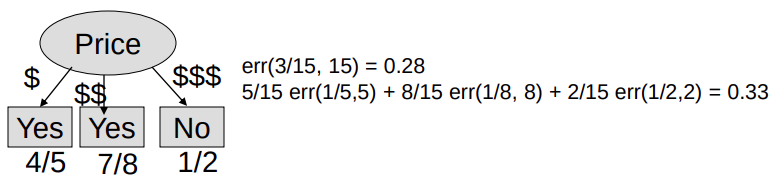
\includegraphics[width=0.65\textwidth]{prune.png}
		\end{figure}
		$\rightarrow$ error rate of the node = 0.28 < combined error rate of the children = 0.33 
		
		$\rightarrow$ prune back, the leaf node is the \textbf{most frequent class}.
	\end{itemize}
	\item Use-case: C4.5, CART, however, computationally expensive
	\item Data for pruning:
	\begin{itemize}
		\item hold-out set: an \textbf{independent} dataset from the training data. Best, but not practical when data is scarce.
		\item training data: Used in C4.5, derive \textbf{outer bound of confidence interval} from data, use a \textbf{heuristic limit} for error rate. If the \textbf{error rate is outside the confidence interval} $\rightarrow$ \textbf{prune} back. 
		
		$\rightarrow$ confidence limit c $\downarrow$ (25\% -> 10\%), the tree prunes \textbf{stronger}.
	\end{itemize}
\end{itemize}




	\section{Ensemble Methods: Regression \& Multinomial Classification}
Ensemble methods can be applied widely, both in \textbf{regression} and \textbf{classification}. We have a slight focus of classification here.
\begin{itemize}
	\item Definition: \textbf{combination of multiple models}. Build and output different ''expert'' models, let them vote for decision. 
	\item Comparison over a \textbf{single model}: 
	\begin{itemize}
		\item a combination of several bad models sometimes achieves better result than a single good model. It ensembles different models with \textbf{low bias and high variance} and may
		\begin{itemize}
			\item reduce overall variance
			\item increase predictive performances
			\item decrease expected error (bias + variance)
		\end{itemize}
		\item ensemble models tend to be \textbf{more stable}, a small change in input data doesn't necessarily change the final prediction.
	\end{itemize}
	\item Types of Ensemble methods:
	\begin{itemize}
		\item Bagging
		\item Random Forest
		\item Boosting
		\item Stacking
	\end{itemize}  
\end{itemize}

\subsection{Bagging}
Bagging randomizes the \textbf{data} in training.
\begin{itemize}
	\item idea: reduces \textbf{variance} of \textbf{low-bias models}.
	\item Training Models (Training)
	\begin{itemize}
		\item randomly sample \textbf{m training subsets} of \textbf{size n} from the whole training data. (sample \textbf{with replacement}) 
		\item train one model for \textbf{each training subset independently} 
	\end{itemize}
	
	\item Classifying Instances (Testing)
	\begin{itemize}
		\item each trained model predicts the test data independently \textbf{with equal weight}.
		\item classification result: the \textbf{most frequent class}
	\end{itemize}
	\item Advantages:
	\begin{itemize}
		\item applied both in numeric prediction and classification
		\item works well when data is \textbf{noisy}
		\item improves performance if the learning scheme is \textbf{unstable} (eg: decision tree)
		\item can be \textbf{parallelized}.
	\end{itemize}
\end{itemize}
\subsection{Random Forest}
Random Forest \textbf{randomizes both data and feature selection}!!
\begin{itemize}
	\item Definition/Process: \textbf{aggregates} full grown trees with \textbf{low bias but high variance}. 
	
	$\rightarrow$ reduce the variance of the final predictor by \textbf{aggregating} all trees.
	\item Training Models:
	\begin{itemize}
		\item define the $n$ number of trees, and the $m$ number of attributes to try.
		\item for each tree, draw a \textbf{bootstrap sample of data} (random sample with replacement), \textbf{randomly select $m$ attributes}.
		\item train each tree with their selected attributes \textbf{independently}.
	\end{itemize}

	\item Classifying Instances:
	\begin{itemize}
		\item each trained model predicts the test data independently (default: with equal weight). 
		\item classification result: aggregate the tree, result is the \textbf{most frequent class}.
		\item \textbf{Weighting possible}. 
	\end{itemize}

\end{itemize}

\subsection{Boosting}
\begin{itemize}
	\item Idea: combines \textbf{weak learners} into a \textbf{strong learner}. 
	
	$\rightarrow$ reduces \textbf{bias} of \textbf{low-variance models}.
	\item Training Models (example: Adaboost):
	\begin{itemize}
		\item Initialization: all training instances have \textbf{equal weight}.
		\item First model:  is trained and predicts \textbf{the training data instances} back.
		\item Evaluation of prediction: \textbf{correct} prediction gets \textbf{lower} weights, \textbf{false} prediction gets \textbf{higher} weights.
		\item \textbf{based on the last model}, repeat step 2-3. Until $m$ models are trained, always focus on traing data \textbf{with high weights} -- misclassified instances. 
	\end{itemize}
	\item Classifying Instances: 
	\begin{itemize}
		\item each model is assigned \textbf{weight according to error rate} from training.
		\item each trained model predicts the test data independently.
		\item classification result: \textbf{weighted average} of classes.
	\end{itemize}
	\item Algorithms: AdaBoost(weighting instances), XGBoost(trained on residual errors), etc.
\end{itemize}

\subsection{Bagging VS. Boosting}
\begin{figure}[H]
	\centering
	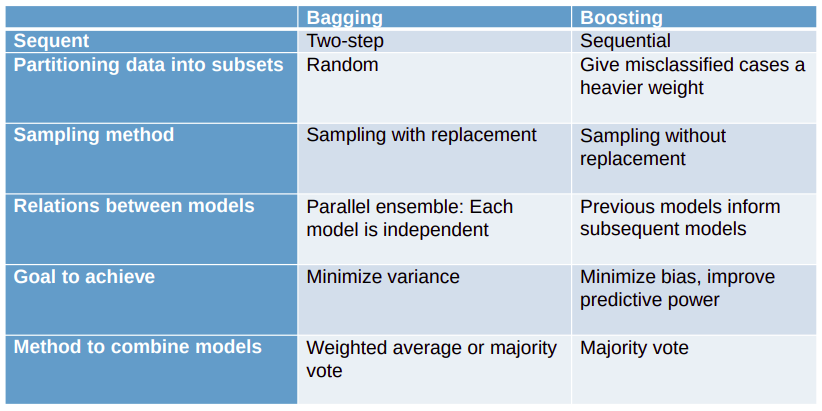
\includegraphics[width=0.85\textwidth]{bagging-boosting.png}
\end{figure}
\subsection{Stacking \& Meta-Learning}
\begin{itemize}
	\item Idea: different level models will be stacked on, predictions from \textbf{different classifiers(level-0 models)} are used as input into a \textbf{meta-learner(level-1 model)}. 
	\item Training Models -- level 0:
	\begin{itemize}
		\item split the training data into \textbf{training subset} and \textbf{holdout subset}.
		\item $m$ different models(NB, DT, etc.) are trained \textbf{independently} on the training subset. 
		
		$\rightarrow$ level-0 classifiers
	\end{itemize}
	\item Classifying Instances -- level 0:
	\begin{itemize}
		\item the level-0 classifiers predicts on \textbf{holdout subset}
		\item the holdout set contains \textbf{only the prediction results of all level-0 classifiers}.
	\end{itemize}
	\item Training Models -- level 1:
	\begin{itemize}
		\item training holdout serves as \textbf{training data} for a \textbf{single} level-1 model (normally simple, eg:regression).
	\end{itemize}
	\item Classifying Instances -- level 1:
	\begin{itemize}
		\item classify the test data with the level-1 model.
	\end{itemize}
\end{itemize}
	\section{Neural Networks: Regression \& Multinomial Classification}
supervised learning. 
\subsection{Terminology}
\paragraph{Training Example} has form ($x_n, y_n$), with $x_n$ as input vector, $y_n$ expected/true output vector.

\paragraph{Loss/Cost Function} maps values of one or more variables onto a number representing \textbf{loss/cost}.

Learning $\rightarrow$ minimizing a loss function.

\paragraph{Risk Function} \textbf{expectation} of the \textbf{loss function}. In neural network, we minimizes our risk by  \textbf{minimizing the empirical risk function -- average loss of all training examples}.

\paragraph{Activation Function} 
\begin{itemize}
	\item linear activation  
	\item sigmoid activation: \textbf{focus of this lecture},  $\sigma(x) = \frac{e^x}{1 + e^x}$
	\item Perceptron activation
	\item ReLU activation
\end{itemize}
\paragraph{Epoch} one \textbf{forward pass} and one \textbf{backward pass} of \textbf{all} training examples. One pass = forward + backward pass.
\begin{itemize}
	\item Forward Pass: calculate the output of \textbf{all training } through the neural network.
	\item Backward Pass: Backpropagation 
\end{itemize}

\paragraph{Backpropagation} calculate a \textbf{gradient} that is needed in \textbf{calculation of weights} to be used in network. It describes how a \textbf{single training example} starting from \textbf{output neurons} determines the goal for the neurons on the next layer and \textbf{steps backwards recursively}.

\paragraph{Multi-Layer Feed-Forward Networks} represent arbitrary \textbf{non-linear} functions. It consists of
\begin{itemize}
	\item input layer
	\item hidden layer with \textbf{activation}
	\item output layer with \textbf{activation}
\end{itemize}
\textbf{Weights and biases} need to be adapted in the neural network. 

$\rightarrow$ updated by \textbf{backpropagation (gradient descent)}.

\subsection{Multi-Layer Feed-Forward Network}
\subsubsection{Setup of a Neural Network}
\begin{figure}[H]
	\centering
	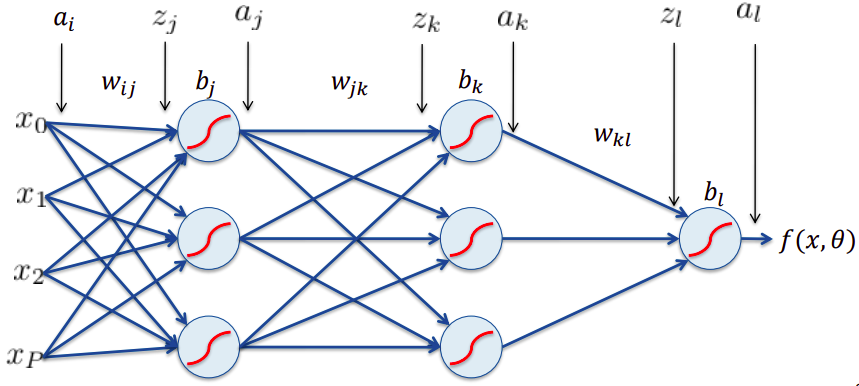
\includegraphics[width=0.7\textwidth]{nn.png}
\end{figure}

\subsubsection{Process}
Goal of training: \textbf{minimizes loss function, minimizes empirical risk}.
\\ \ \\
Assume a network with 1 hidden layer, 1 output layer:

\begin{enumerate}[label= \protect \circled{\arabic*} ]
	\item \textbf{Forward Pass}: from input layer to output layer (with \textbf{sigmoid} activation).
	
	If we are asked to perform, this calculation can done \textbf{matrix-wise}!! No need to separate each observation.
	
	\begin{align*}
		z^{[1]} &= W^{[1]}\cdot a^{[0]} + b^{[1]} =  W^{[1]}\cdot x + b^{[1]}\\
		a^{[1]} &= g^{[1]}(z^{[1]}) = \sigma(z^{[1]}) \\
		z^{[2]} &= W^{[2]}\cdot a^{[1]} + b^{[2]} \\
		a^{[2]} &= g^{[2]}(z^{[2]}) = \sigma(z^{[2]})
	\end{align*}
	
	\item \textbf{Loss Function}: calculate the loss of the network output according to the loss function $l(y, \hat{y})$
	
	If we evaluate the model using \textbf{cross-entropy loss}: the calculation for $y \ln\hat{y}$ is a dot product(element-wise multiplication).
	$$l(y,\hat{y}) = - [y \ln \hat{y} + (1-y)\ln(1 - \hat{y})]$$
	\item \textbf{Empirical Risk}: calculate the empirical risk $\mathcal{L}$ by \textbf{averaging} the loss.
	$$\mathcal{L}(y,\hat{y}) = \frac{1}{n} \cdot \Sigma l(y,\hat{y})$$
	
	\item \textbf{Backpropagation}: readapt the \textbf{weights and biases} using \textbf{gradient descent}. 
	
	example in updating layer 2:
	\begin{align*}
		W^{[2]}_{t+1} &= W^{[2]}_t - \alpha \cdot dW =W^{[2]}_t - \alpha \cdot \frac{\partial L}{\partial W^{[2]}} \\
		b^{[2]}_{t+1} &= b^{[2]}_t - \alpha \cdot db =b^{[2]}_t - \alpha \cdot \frac{\partial L}{\partial b^{[2]}} 
	\end{align*}
	\begin{itemize}
		\item $\frac{\partial L}{\partial W^{[2]}}, \frac{\partial L}{\partial b^{[2]}}$: chain rule
		$$\frac{\partial L_n}{\partial W} = \frac{\partial L_n}{\partial a_{n}} \cdot \frac{\partial a_{n}}{\partial z_{n}} \cdot \frac{\partial z_n}{\partial W}$$
	\end{itemize}
	\begin{align*}
		L_n &= \frac{1}{2} (y_{n} - g(w_{kl}a_{kn} + b_l))^2 = \frac{1}{2} (y_n - a_{ln})^2, \quad &\frac{\partial L_n}{\partial a_{ln}} &= -(y_n - a_{ln})\\
		a_{ln} &= g(z_{ln}) , \quad &\frac{\partial L_n}{\partial z_{ln}} &= g'(z_{ln}) \\
		z_{ln} &= w_{kl}a_{kn} + b_l, \quad &\frac{\partial L_n}{\partial w_{ln}} &= a_{kn} 	
	\end{align*}

	If the activation is a sigmoid activation: $\sigma(x) = \frac{e^x}{1 + e^x}$, $\sigma'(x) = \sigma(x)(1 - \sigma(x))$.
	$$dW^{[2]} = -(y- a^{[2]})\cdot a^{[1]^{T}} = (a^{[2]} - y) \cdot a^{[1]^{T}}$$
\end{enumerate}

\subsubsection{Trainable Parameters}
Number of trainable parameters: the \textbf{free parameters} of the neural network are \textbf{weights and biases}-- $W^{[1]}, b^{[1]}, W^{[2]}, b^{[2]}, \dots$. 

$\rightarrow$ define the \textbf{dimension} of these parameters, add up all possible trainable elements. 

(eg: $W^{[1]}$ is 2x2-matrix, therefore 4 trainable parameters)
\subsection{Gradient Descent for Backpropagation}
\begin{itemize}
	\item Goal: given any function f, find $x^* = \arg\min_{x} f(x)$
	\item \textbf{Gradient} at position x is defined as the \textbf{partial derivative}: 
	$$\nabla f(x) = \begin{bmatrix}
	\frac{\partial f(x)}{x_1} \\ \vdots \\ \frac{\partial f(x)}{x_d}
	\end{bmatrix}$$ 
	\begin{itemize}
		\item Interpretation: in d-dimensional space, gradient points in \textbf{direction of steepest ascent} of f at point x. 	
	\end{itemize}
	$\rightarrow$ to \textbf{minimize loss function} $\rightarrow$ \textbf{descent}, the opposite direction $\mathbf{- \nabla f(x)}$.
	
\end{itemize}
\subsubsection{General Process}
\begin{enumerate}[label= \protect \circled{\arabic*} ]
	\item choose an \textbf{initial point}
	\item choose a \textbf{step size (either fixed or dynamic)}.
	\item take a step in the \textbf{direction opposite the gradient}.
	\begin{itemize}
		\item fixed step size:
		$$\begin{bmatrix}
		x_n \\y_n
		\end{bmatrix} = \begin{bmatrix}
		x_{n-1} \\ y_{n-1}
		\end{bmatrix} - \alpha \cdot \nabla f(x_{n-1}, y_{n-1})$$
		\item dynamic step size:
		$$\begin{bmatrix}
		x_n \\y_n
		\end{bmatrix} = \begin{bmatrix}
		x_{n-1} \\ y_{n-1}
		\end{bmatrix} - \alpha_{n} \cdot \nabla f(x_{n-1}, y_{n-1})$$
	\end{itemize}
	\item repeat till convergence.
\end{enumerate}

Convergence to optimum: depends on the \textbf{step size}. 
\begin{itemize}
	\item too small: would converge eventually, but takes long time.
	\item too large: value \textbf{oscillates}, doesn't converge.
	\item would stall if $\nabla f(x) = 0$. 
	\item can stuck at saddle point.
\end{itemize}
Criteria: 
\begin{itemize}
	\item function f is \textbf{convex}
	\item step size $\alpha$ is square summable, but not summable.
\end{itemize}
$\rightarrow$ Alternative: introduce \textbf{momentum}.

\subsubsection{Process with Momentum Introduced}
\begin{itemize}
	\item Idea: uses an exponential averaging of gradients to \textbf{make sudden changes in direction less likely}.
\end{itemize}
\begin{align*}
	d_n &= \beta \cdot d_{n-1} + \alpha \cdot\nabla f(x_{n-1})\\
	x_n &= x_{n-1} - d_n
\end{align*}

	\section{Causal Inference}
Given a \textbf{treatment}, we want to know if there is a \textbf{causality} between the \textbf{treatment and outcome}.

Given a \textbf{control group} and \textbf{treatment group}, if we can observe the before and after treatment for both groups, we can find out different treatment effects:
\begin{itemize}
	\item individual treatment effect: $Y_{1i} - Y_{0i}$
	\item average treatment effect: $E(Y_{1i} - Y_{0i})$
	\item subgroup treatment effect: $E(Y_{1i} - Y_{0i} | X)$
\end{itemize}
However, $Y_{1i}$ and $Y_{0i})$ can't be both observable for one group.

$\rightarrow$ approximation

\subsection{Data Collection in Causal Inference}
\paragraph{Golden Rule} \textbf{randomized controlled trials}. The treatment is controlled, individuals are assigned randomly to the treatment. 

$\rightarrow$ Sample selection bias is prevented.

\subsubsection{Different Types of Experiments/Data Collections}
\begin{itemize}
	\item \textbf{Randomized Controlled Trials}: Treatment/Control groups separated. Subject is \textbf{randomly assigned} to the \textbf{treatment/control} group.
	
	$\rightarrow$ minimum selection bias
	\begin{itemize}
		\item Lab Experiments
		\item Field Experiments
	\end{itemize}
	
	\item \textbf{Quasi-experiements}: \textbf{natural groups} pre-exist, no separation of control/treatment group beforehand. The independent variable(treatment variable) is \textbf{controlled}, subjects are \textbf{not randomly assigned}.
	
	$\rightarrow$ selection bias
	
	\item \textbf{Observational studies}: what we always have. The independent variable is \textbf{not controlled}, individuals \textbf{self-assigned}.
	
	$\rightarrow$ selection bias 
	\begin{itemize}
		\item cross-sectional study
		\item longitudinal study
		\item panel study
		\item case-control study
	\end{itemize}
\end{itemize}

\subsection{Challenges to Quasi-Experiments \& Observational Studies: Confounding Variables \& Identification Strategies}
\subsubsection{Confounding Variables}

 For \textbf{Quasi-Experiments and Observational Studies}, confounding variables might exist, but \textbf{not observable, therefore omitted from the model}. In order to identify precise causal effects, we need to deal with confounding variables.


\paragraph{Confounding Variables} an extraneous variable that is \textbf{unobservable}, which \textbf{correlates} with \textbf{dependent and independent variables}.

$\rightarrow$ $Cov(\varepsilon, X) \neq 0$ $\rightarrow$ Endogeneity

$\rightarrow$ Consequence: biased results.

\subsubsection{Combat Confounding Variables by Data Collection: Randomized Controlled Trials}
Apply Randomized Controlled Trials: confounding variables \textbf{automatically removed}.

Ways to conduct RCTs:
\begin{itemize}
	\item Lab experiment
	\item Field experiement
\end{itemize}
\begin{figure}[H]
	\centering
	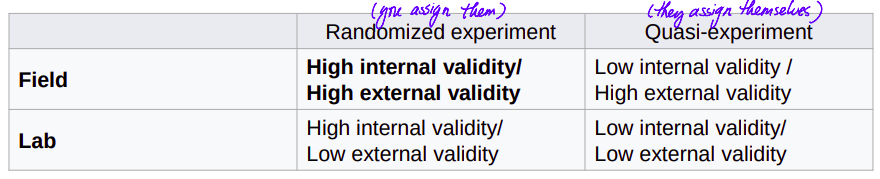
\includegraphics[width=0.8\textwidth]{labfield.png}
\end{figure}
\subsubsection{Indentification Strategy for Quasi-Experiments: Difference-in-Difference}
\begin{itemize}
	\item Idea: Observe the \textbf{effect of treatment} controlled by the researcher between \textbf{control \& treatment group}, \textbf{over time}. 
	\item Process:
	\begin{itemize}
		\item Assume there exists an \textbf{overall trend} on both control \& treatment group. We still want to estimate the treatment effect while not omitting confounding variable (eg: time). 
		\item treatment effect:
		$$\text{Treatment effect} = (Y_{t2} - Y_{t1}) - (Y_{c2} - Y_{c1})$$
	\end{itemize}
\end{itemize}




\subsubsection{Indentification Strategy for Panel Studies: Fixed-Effect Models}
\begin{itemize}
	\item Idea: \textbf{Fixed influence} is omitted as one of the confounding variables in modeling the treatment effect on outcome.
	
	$\rightarrow$ model \textbf{fixed effect} to soak up \textbf{individual effects on model}.
	\item Fixed-Effect Model: the fixed effect is modeled as an \textbf{additional intercept $\lambda_i$} for \textbf{each individual}.
\end{itemize}

\subsubsection{Indentification Strategy for Observational Studies: Propensity Score Matching}
\begin{itemize}
	\item Idea: in cross-sectional data, find a \textbf{data section} where control \& treatment group has the \textbf{maximum similarity} in covariate distribution. 
	
	$\rightarrow$ resembles \textbf{randomized experiment}
	
	\item Process:
	\begin{itemize}
		\item estimate \textbf{propensity score} by logistic regression for each individual in \textbf{treatment group}. 
		\item \textbf{match} the \textbf{control group} to the treatment group. Find subjects with \textbf{similar propensity score}.
		\item evaluate quality of matching
		\item evaluate \textbf{treatment effect} based on the \textbf{treatment and matched control group}.
		
	\end{itemize}
\end{itemize}

\subsubsection{Confounding Variable as Instrument Variables}
\paragraph{Instrument} attributes that \textbf{has causal effect} on \textbf{treatment variable}, but \textbf{no causal effect} on \textbf{outcome}.
\begin{itemize}
	\item Modeling Process:
	\begin{itemize}
		\item instruments \textbf{randomly assigned} to the treatment variable
		\item model the relationship between the instrument and treatment variable.
		\item model the relationship between the predicted treatment variable and outcome.
	\end{itemize}
	\item Estimation: 2-stage least square.                                                                                                                                                                                   
\end{itemize}


	\newpage
\part{Unsupervised Learning}
\section{Clustering}
\begin{itemize}
	\item Definition: given a database $D = {t_1, \dots, t_n}$ of tuples and an integer value $k$, define a mappping $f: D \rightarrow {1, \dots, k}$ where each tuple $t_i$ is assigned to a cluster $K_j$.
	\item Input: a dataset with $n$ p-dimensional data instances.
	
	Output: a \textbf{natural partitioning} of the dataset into $k$ clusters and noise
	\item Clustering VS. Classification
	\begin{table}[H]
		\begin{center}
			\begin{tabular}{|l|p {0.3\linewidth}|p {0.35\linewidth}|}
				\hline
				Characteristics        & \textbf{Classification}  & \textbf{Clustering}   \\ \hline
				Learning     & supervised  & unsupervised \\ \hline
				Target       & known & unknown, no dependent variables \\ \hline
				Training  	 & training data and training phase exists  & no training data/training phase, no labels/true classes  \\ \hline
			\end{tabular}
		\end{center}	
	\end{table}
	\item key questions: 
	\begin{itemize}
		\item the right number of clusters k
		\item identification of class membership between instances
	\end{itemize}
	\item Issues:
	\begin{itemize}
		\item interpreting results
		\item evaluating results: high intra-similarity within cluster, low inter-similarity across cluster? 
		\item outlier
		\item number of clusters k
		\item scalability of algorithms
	\end{itemize}
\end{itemize}

\subsection{Hierarchical Clustering : Minimum Spanning Tree}
\begin{itemize}
	\item Input: a database D with tuples, \textbf{adjacency matrix} based on distances
	
	Output: \textbf{dendogram}
	\item Methods of building a dendogram: 
	\begin{itemize}
		\item top-down
		\item bottom-up
	\end{itemize}
	\item Algorithms: with adjacency matrix, \textbf{each instance} can be seen as \textbf{node}, \textbf{distance} to other instances can be seen as \textbf{weighted edges} 
	
	$\rightarrow$ graph problem
	
	$\rightarrow$ compute \textbf{Minimum Spanning Tree}, bottom-up method.
	\begin{itemize}
		\item Kruskal's algorithm: $\mathcal{O}(d\log(d))$
		\item Prim's algorithm: $\mathcal{O}(d\log(n))$
	\end{itemize}
	$\rightarrow$ each hierarchical level shares the same distance/weight.
	
	\item Distance measures in adjacency matrix:
	\begin{itemize}
		\item \textbf{Euclidean distance} between instance $p_1$ and $p_2$
		$$d_E(p_1,p_2) = \sqrt{(x_{p1} - x_{p2})^2 + (y_{p1} - y_{p2})^2 +\dots }$$
		\item \textbf{Manhattan distance} between instance $p_1$ and $p_2$
		$$d_M(p_1,p_2) = |x_{p1} - x_{p2}| + |y_{p1} - y_{p2}| + \dots$$
	\end{itemize}
\end{itemize}

\subsection{Partitional Clustering for Numeric Data: K-Means}
\begin{itemize}
	\item Input: 
	\begin{itemize}
		\item a database D with tuples
		\item $k$ number of clusters
	\end{itemize}
	 
	Output: k partitioned clusters
	\item Process:
	\begin{itemize}
		\item Initialization: randomly picked k centers
		\item compute the distance between each instance to the centers, assign instance to the \textbf{nearest center}.
		\item \textbf{update} the center of the clusters: \textbf{mean of assigned instances}
		\item repeat step 2-3 until convergence.
	\end{itemize}

	\item Advantages:
	\begin{itemize}
		\item simple
		\item items automatically assigned to clusters
	\end{itemize}
	Disadvantages:
	\begin{itemize}
		\item number of clusters $k$ must be predefined
		\item result significantly depends on \textbf{initial choice of centers} 
		
		$\rightarrow$ traps in \textbf{local minimum} 
		
		$\rightarrow$ repeat algorithm by starting from different random centers (eg: Iterative Improvement)
		\item sensitive to \textbf{outliers}
	\end{itemize}
\end{itemize}

\subsection{Probabilistic Clustering: Expectation Maximization}
We only discuss the simplified case here: instance with single \textbf{numeric} attribute and 2 clusters A \& B.
\begin{itemize}
	\item Input: random assigned parameters for cluster A \& B, assume \textbf{normal distribution}
	\begin{itemize}
		\item A: $\mu_A, \sigma_A$, prior probability of instance in cluster A $Pr(A)$
		\item B: $\mu_B, \sigma_B$, prior probability of instance in cluster B $Pr(B) = 1 - Pr(A)$
	\end{itemize}
	Output: 2 clusters with assigned instances
	
	\item Process:
	\begin{itemize}
		\item \textbf{Expectation} step: calculate the probability for \textbf{all instances} in \textbf{each cluster}: \textbf{Bayes Theorem}
			$$Pr(A|x) = \frac{Pr(x|A) \cdot Pr(A)}{Pr(x)} ,\quad Pr(x|A) = \frac{1}{\sqrt{2\pi} \cdot \sigma_A} e^{-\frac{(x - \mu_A)^2}{2\sigma_A^2}}$$
			$$Pr(B|x) = \frac{Pr(x|B) \cdot Pr(B)}{Pr(x)} ,\quad Pr(x|B) = \frac{1}{\sqrt{2\pi} \cdot \sigma_B} e^{-\frac{(x - \mu_B)^2}{2\sigma_B^2}}$$
		\textbf{no need to pick cluster here!}
		\item \textbf{Maximization} step: update the parameters for cluster A \& B. calculate the weighted mean and weighted variance using \textbf{all instances}. 
		$$w_{iA} = Pr(A|x), \quad  w_{iB} = Pr(B|x)$$
		$$\mu_A = \frac{w_{1A}x_1 + w_{2A}x_2 + \dots + w_{nA}x_n}{w_{1A} + w_{2A} + \dots + w_{nA}}$$
		$$\sigma_A = \sqrt{\frac{w_{1A} (x_1 - \mu_A)^2 + \dots + w_{nA} (x_n - \mu_A)^2}{w_{1A} + w_{2A} + \dots + w_{nA}}}$$
		analog to $\mu_B$ and $\sigma_B$
		
		$$Pr(A) = \frac{\Sigma w_A}{\Sigma w_A + \Sigma w_B}, \quad Pr(B) = 1 - Pr(A)$$
		\item repeat expectation and maximization step until convergence.
	\end{itemize}
	\item Limitation: can stuck in \textbf{local optimum}. 
	
	$\rightarrow$ repeat algorithm by starting with \textbf{different initial parameters}.
	
	\item Extension of model:
	\begin{itemize}
		\item multiple clusters: calculate k normal distributions
		\item multiple attributes: 
		\begin{itemize}
			\item independent: multiply probabilities of all attributes
			\item correlated: multivariate normal distribution
		\end{itemize}
		\item nominal attributes: create probability distribution
	\end{itemize}
\end{itemize}
	\section{Association Rules Discovery}
\begin{itemize}
	\item Goal: discover \textbf{correlation among attributes} or other relationships in large databases.
	\item Use-case: Market Basket Analysis, cross/up-selling
	\item \textbf{Unsupervised learning}: no dependent variable defined, no labeled training data.
\end{itemize}

\subsection{Terminology}

\paragraph{Rule} if $A$ and $B$ then $C$ and $D$. denote as $R: A,B \Rightarrow C,D$. It only describes \textbf{correlation}, not causality. 



\paragraph{Transaction Database} an instance/observation is a transaction. Each \textbf{attribute} in the database is converted to \textbf{binary flags 0/1}. 
\paragraph{Item} single element/attribute. eg: Milk/Bread
\paragraph{Itemset} a set of items. eg: {Milk, Bread, Butter}
\paragraph{Frequent Itemset} the itemset $I$ that meets the \textbf{minimum support}. $$supp(I) \geq \min supp$$
\paragraph{Support}
\begin{itemize}
	\item support of \textbf{an item set}: \textbf{relative frequency} of the transactions that contain the item-set in \textbf{all transactions}
	\item support of \textbf{a rule}: the support of all item sets it contains. 
	$$supp(A,B \Rightarrow C,D) = supp(\{A,B,C,D\})$$
	The \textbf{order, the arrow} of the rule \textbf{doesn't matter in computing support}.
	$$supp(\text{Milk} \Rightarrow \text{Bread}) = supp(\{\text{Milk, Bread}\}) = supp(\{\text{Bread} \Rightarrow \text{Milk}\})$$
	
	\item support \textbf{estimation}: lower bound + upper bound. 
	\begin{itemize}
		\item lower bound: the support of a subset is always higher than its superset. \textbf{subset property}, every subset of a frequent set is frequent. 
		$$supp(\{B,C\}) \geq supp(\{A,B,C,D\})$$
		\item upper bound: use Venn-Diagramm.
	\end{itemize}
\end{itemize}

\paragraph{Confidence of a Rule} the likeliness to apply to the dataset. $\rightarrow$ the probability that X and Y coexist given that X exists.
$$conf(R: X \Rightarrow Y) = \frac{supp(X \cup Y)}{supp(X)}$$

$$conf(\{\text{Milk,Bread}\} \Rightarrow \{\text{Butter}\}) = \frac{supp(\{\text{Milk, Bread, Butter}\})}{supp(\{\text{Milk, Bread}\})}$$

\paragraph{Strong Rule} association rules with \textbf{minimum support \& confidence}.

\paragraph{Lift of a Rule} indicates \textbf{by how much (ratio)} the \textbf{confidence of a rule} surpasses the \textbf{expected value}. 
$$Lift(R: X \Rightarrow Y) = \frac{conf(R)}{expConf(R)} = \dfrac{\frac{supp(X \cup Y)}{supp(X)}}{supp(Y)} = \frac{supp(X \cup Y)}{supp(X)\cdot supp(Y)}$$

\subparagraph{Interpretation of Lifts}
\begin{itemize}
	\item lift < 1: X has \textbf{positive} effect on Y. Item-sets X and Y appears \textbf{more frequent than expected value}.
	\item lift = 1: X and Y are \textbf{independent}. X has \textbf{no effect} on Y.
	\item lift > 1: X has \textbf{negative} effect on Y. Item-sets X and Y appears \textbf{less frequent than expected value}.
\end{itemize}


\subsection{A priori Algorithm: Generation of Itemsets and Rules}

\begin{itemize}
	\item Idea: if X is a frequent k-item set, then all (k-1)-item subsets of X have to be frequent item sets as well.
	
	$\rightarrow$ iteratively compute frequent item sets, compute k-item sets by merging (k-1)-item sets.
	
	\item Process: 
	\begin{enumerate}[label= \protect \circled{\arabic*} ]
		\item Generation of \textbf{Item sets}: 
		\begin{itemize}
			\item start with item sets in \textbf{size 1}.
			\item only select those that \textbf{exceeds minimum support} $\rightarrow$ frequent.
			\item iteratively build item sets in larger sizes based on previous sizes. 
		\end{itemize}
	\begin{figure}[H]
		\centering
		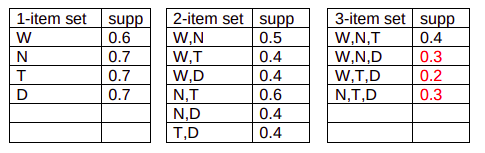
\includegraphics[width=0.5\textwidth]{itemset.png}
	\end{figure}
		\item Generation of \textbf{Rules} based on frequent item sets:
		\begin{itemize}
			\item start with rules with only \textbf{1 item on the right}. 
			\item rule $X \Rightarrow Y$ is different from $Y \Rightarrow X$. Compute \textbf{both directions}. 
			\item only select rules that \textbf{exceeds minimum confidence}. 
			\item evaluate rules containing \textbf{multiple items on the right} by checking whether single item on the right side. \textbf{Only expand if single rules exceeds minimum confidence.}
			$$X \Rightarrow Y, Z \quad \text{bases on} \quad X \Rightarrow Y \quad \text{and} \quad X \Rightarrow Z$$ 
		\end{itemize}
	\begin{figure}[H]
		\centering
		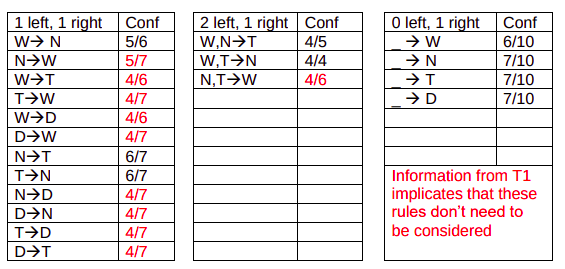
\includegraphics[width=0.6\textwidth]{ruleset.png}
	\end{figure}
	\end{enumerate}
\end{itemize}

\section{Recommendation Systems}
\begin{itemize}
	\item Approaches:
	\begin{itemize}
		\item Association Rules: discover \textbf{correlations}
		\begin{itemize}
			\item product association
			\item user association
			\item combination of both
		\end{itemize}
		\item Collaborative Filtering: discover \textbf{similarity}
		\item Singular Value Decomposition
	\end{itemize}
\end{itemize}

\subsection{Collaborative Filtering}
\begin{itemize}
	\item Idea: 
	\begin{itemize}
		\item maintain a database of \textbf{user's rating} on items.
		\item for a \textbf{given active user}, find other \textbf{similar users} whose \textbf{rating strongly correlates} with the active user.
		
		$\rightarrow$ recommend items highly rated by similar users, which is \textbf{not rated} by active user.
	\end{itemize}
	
\end{itemize}

\subsubsection{Process}
\begin{enumerate}[label= \protect \circled{\arabic*} ]
	\item define \textbf{active user} $a$ and \textbf{other users} $u$.
	\item calculate \textbf{weighted correlation} $w_{a,u}$ based on \textbf{number of co-rated items m} . 
	\begin{itemize}
		\item calculate average of the \textbf{co-rated items} $\bar{r}_a, \bar{r}_u$
		\item calculate the variance $\sigma_{r_{a}}^2, \sigma_{r_{u}}^2$ and standard deviation.
		\item calculate the covariance. \textbf{Don't forget the minus/plus symbol!!!} 
		\item calculate the weighted correlation.
	\end{itemize}
	
	$$w_{a,u} = s_{a,u} \cdot c_{a,u}$$ 
	$$c_{a,u} = \frac{Cov(r_{a}, r_{u})}{\sigma_{r_{a}} \cdot \sigma_{r_{u}}}$$
	$$Cov(r_{a}, r_{u}) = \frac{1}{m-1}\cdot \Sigma (r_a - \bar{r}_a) (r_u - \bar{r}_u)$$
	\item \textbf{rating prediction} for item i for active user.
	\begin{itemize}
		\item calculate \textbf{average rating for all rated items} $\bar{r}_a$ of active user a. 
		\item calculate \textbf{average rating for all rated items} $\bar{r}_u$ of each other user u.
		\item $r_{u,i}$: other user u's rating on the i-th item.
	\end{itemize}
	$$p_{a,i} = \bar{r}_a + \Sigma_{u = 1}^k \dfrac{w_{a,u} \cdot (r_{u,i} - \bar{r}_u)}{\Sigma_{u=1}^k |w_{a,u}|}$$
\end{enumerate}	

\subsubsection{Limitation in Collaborative Filtering}
\begin{itemize}
	\item \textbf{Cold Start}: \textbf{enough users and ratings} are needed to generate recommendations.
	\item \textbf{Sparsity}: the user/rating matrix can be sparse even there are many users 
	
	$\rightarrow$ hard to find \textbf{co-rated} items.
	\item \textbf{First Rater}: with a \textbf{new product}, there must first be consumers who test and evaluate it. 
	\item \textbf{Popularity Bias}: cannot recommend items to users with \textbf{unique taste}. Tend to recommend popular items.
\end{itemize}

$\rightarrow$ Alternative: \textbf{Content-Based Filtering}
\begin{itemize}
	\item idea: based on information of the content of items.
	\item solve: 
	\begin{itemize}
		\item combat popularity bias
		\item combat first rater.
		\item no need of user ratings $\rightarrow$ cold start + sparsity combated.
	\end{itemize}
\end{itemize}

\subsection{Singular Value Decomposition}
\begin{itemize}
	\item Idea: produce a low-dimensional representation of the customer-product space.
	\item Model:
	$$A = U \cdot S \cdot V^T$$
	\begin{itemize}
		\item A: the rating matrix, or the rating we want to predict.
		\item U: maps \textbf{users to concepts}
		\item S: strength of concepts/categories
		\item $V^T$: maps \textbf{venues/products to concepts} 
	\end{itemize}
	\item \textbf{Rating Prediction}: rating for item i from user.
	\begin{itemize}
		\item calculate/consider the average rating of user.
	\end{itemize}
	$$r_{u,i} = \bar{r}_u + U(user) \cdot S \cdot V^T(item)$$
	
	\item Interpretation of values:
	\begin{itemize}
		\item User matrix(U):
		\begin{itemize}
			\item positive: higher interest
			\item negative: lower interest
			\item 0: no interest
		\end{itemize}
		\item Product matrix($V^T$):
		\begin{itemize}
			\item positive: \textbf{positively represented} in the i-th latent factor. Users having preference in i-th latent factor will \textbf{prefer items with positive value over items with negative values}.
			\item negative: \textbf{negatively represented} in the i-th latent factor. Users having preference in i-th latent factor will \textbf{like item less}.
		\end{itemize}
	\end{itemize}
\end{itemize}

	\newpage
\part{CRISP-DM Process Model}
The knowledge discovery process follows the following diagram: \textbf{Data Understanding -- Data Preparation -- Modeling -- Evaluation}. 
\begin{figure}[H]
	\centering
	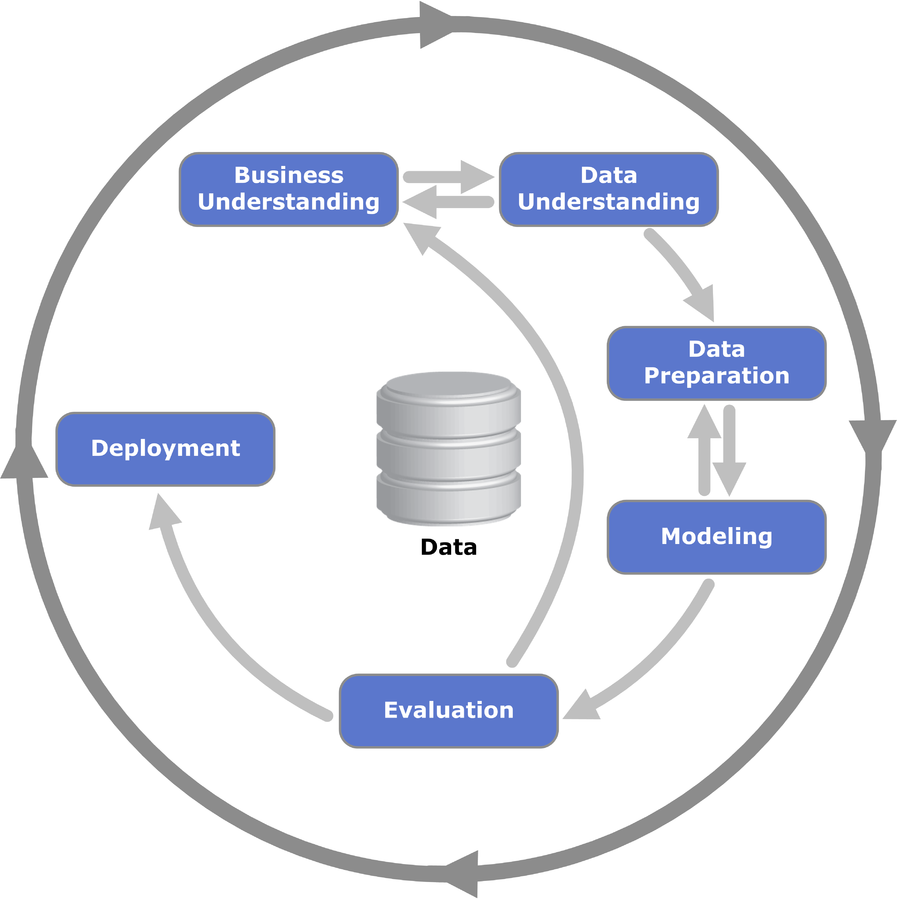
\includegraphics[width=0.45\textwidth]{CRISP-DM.png}
\end{figure}
\section{Data Understanding}
\subsection{Qualitative \& Quantitative Understanding}
Given a dataset description or an attribute table, 
\begin{itemize}
	\item Qualitative understanding:
	\begin{itemize}
		\item format of the data: \textbf{tidy data}?
		\item dependent \& independent variables
		\item scale of measurement of attributes: nominal/ordinal/interval/ratio
		\item cross-sectional, time-series, panel data?
	\end{itemize}
	\item Quantitative understanding
	\begin{itemize}
		\item \# instances, ideal: > 5000
		\item \# attributes, ideal start: < 50
		\item \# targets (balance of classes), ideal: > 100 each class
	\end{itemize}
\end{itemize} 
Ways to obtain understanding:
\begin{itemize}
	\item Visualization: histogram, distribution, relationship between attribute and response
	\item Summary: mean, median, attribute relationships
\end{itemize}

\subsection{Format of Data: tidy?}
\paragraph{Tidy Data} tabular data is tidy if
\begin{itemize}
	\item each \textbf{variable/feature} is in \textbf{single column}
	\item each \textbf{observation/instance} is in \textbf{single row}
	\item each \textbf{value} is in \textbf{single cell}.
\end{itemize}
\begin{figure}[H]
	\centering
	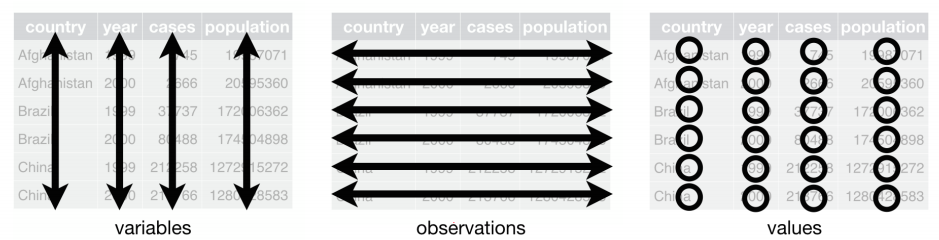
\includegraphics[width=\textwidth]{tidy.png}
\end{figure}
example of tidy data:
\begin{figure}[H]
	\centering
	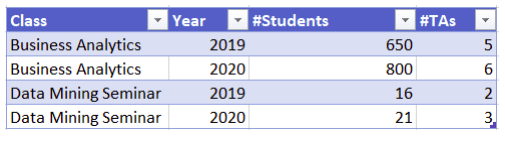
\includegraphics[width=0.6\textwidth]{tidy1.png}
\end{figure}
\paragraph{Wide Data} \textbf{same variable} is spanned into \textbf{multiple columns}. eg: year.
\begin{figure}[H]
	\centering
	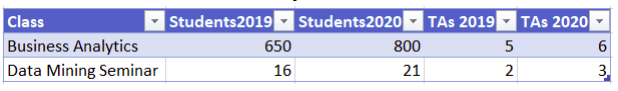
\includegraphics[width=0.7\textwidth]{wide.png}
\end{figure}
\paragraph{Long Data} \textbf{multiple variables} is compressed into \textbf{one column}. eg: n\_Students \& n\_TAs.
\begin{figure}[H]
	\centering
	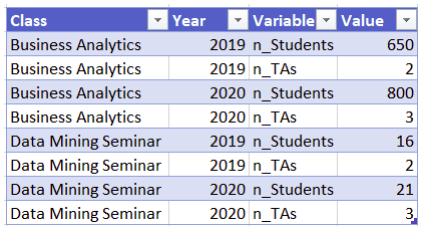
\includegraphics[width=0.5\textwidth]{long.png}
\end{figure}

\section{Data Preparation}
According to the data understanding, we distribute the data preparation also into these 3 parts.

But first of all, \textbf{tidy} the data if the format is long/wide. $\rightarrow$ pivoting.

The data preparation works on tidy data.
\subsection{Instance: Missing Value?}
Missing values need to be \textbf{standardized}:
\begin{itemize}
	\item \textbf{ignore} instance with missing values
	\item treat missing values as \textbf{separate value}
	\item \textbf{imputation}: mean/median
\end{itemize}
\subsection{Attributes: Conversion, Discretization \& Feature Selection}
\subsubsection{Conversion}
\begin{itemize}
	\item ordinal $\rightarrow$ numbers, preserving \textbf{natural order}.
	\item nominal 
	\begin{itemize}
		\item \#attribute values is small: nominal $\rightarrow$ numeric, \textbf{each attribute value} becomes a single \textbf{binary attribute} (number of binary classes: \textbf{(\#attributevalues - 1)} per attribute).
		\item \#attribute values is large: ignore (eg: IDs)
	\end{itemize}
	\item continuous numeric: Discretization, only if model requires(eg: naive Bayes).
\end{itemize}

\subsubsection{Discretization / Binning}
\begin{itemize}
	\item Reasons for Discretization:
	\begin{itemize}
		\item data: numeric data not normally distributed, data requires sorting frequently(decision tree).
		\item model: model requires nominal data as input(naive Bayes).
	\end{itemize}
	\item Reasons against Discretization:
	\begin{itemize}
		\item in decision tree: equi-depth bins \textbf{doesn't maximize the information gain}. Through the algorithm(binary split) we can find better splits instead of binning.
		\item will potentially \textbf{lose ordinal information}.
		\item model-dependent: regression models requires numeric data, no discretization.
	\end{itemize}
	\item Ways of Discretization:
	\begin{itemize}
		\item equi-frequency/depth
		\item class dependent: when decision tree classifier is used, \textbf{best split} according to \textbf{information gain}.
		\item order-preserving: numeric $\rightarrow$ k nominal $\rightarrow$ $(k-1)$ binary attributes, explaining comparison between $(i-1)$ and $i$.
	\end{itemize}
\end{itemize}
\subsubsection{Feature Selection}
\begin{itemize}
	\item Goal: choose the \textbf{most relevant subset}.
	\item Methods:
	\begin{itemize}
		\item Best Subset (search all, select best)
		\item Forward Selection (bottom-up)
		\item Backward Elimination (top-down)
		\item Stepwise Regression (combines forward/backward)
	\end{itemize}
	\item Use-Case: linear regression, classification, dimensionality reduction, regularization
	\item Ideal: at most 50.
\end{itemize}
\subsection{Targets: Balanced Train \& Test Set}
According to the distribution of targets, build up \textbf{balanced set} and then split into \textbf{balanced train set} and \textbf{balanced test set}. 
\begin{itemize}
	\item targets are balanced: each set gets \textbf{same amount} of targets
	\item targets are \textbf{unbalanced}: split \textbf{proportionally}.
\end{itemize}
This only applies to training \& fitting models. It doesn't apply to statistical inference.


	\section{Model Selection}
\subsection{Bias-Variance Tradeoff \& Sweet Spot}
\paragraph{Bias} error from \textbf{erroneous assumptions} in learning algorithm. Error can range from inaccurate assumption to simplification of model.
\paragraph{Variance} error from \textbf{sensitivity to small fluctuations} in training set.
\begin{itemize}
	\item Idea: 
	\begin{itemize}
		\item models \textbf{too simple} will have \textbf{high bias} on training data, \textbf{low variance} on test data.  $\rightarrow$ \textbf{Underfitting}
		\item models \textbf{too complex} will have \textbf{low bias} on training data, \textbf{high variance} on test data. $\rightarrow$ \textbf{Overfitting}
	\end{itemize}
	
	$\rightarrow$ find the sweet spot $\rightarrow$ \textbf{low bias \& low variance}
	
	\item \textbf{Goal} of Model Selection: \textbf{optimize} bias-variance tradeoff
	\item Criterion Metrics: \textbf{minimize} f(fitting error from given data) + g(model complexity)
	\begin{itemize}
		\item \textbf{Akaike Information Criterion(AIC)}: $AIC = -2\ln(L) + 2\cdot \#parameters$
		\item \textbf{Minimum Description Length} given the same quality: Kolmogorov Complexity
	\end{itemize}
\end{itemize}
\begin{figure}[H]
	\centering
	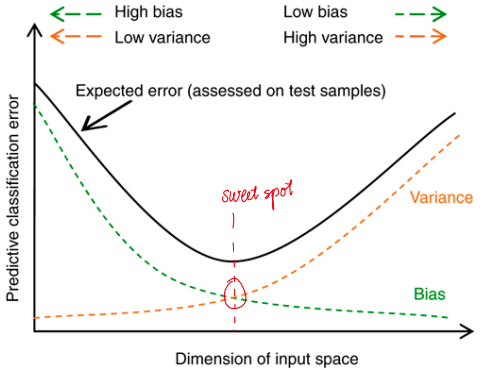
\includegraphics[width=0.5\textwidth]{bias-variance.png}
\end{figure}

\section{Evaluation}
\subsection{Evaluation Methods of Model}
\begin{itemize}
	\item Goal of evaluation: how good is the model on \textbf{new data}?
	\item Evaluation methods: how to get the \textbf{test data}?
	\begin{itemize}
		\item on training set
		\item Holdout set (stratified / repeated)
		\item k-Fold Cross-Validation (w/o stratified)
		\item Leave-One-Out Validation 
		\item Bootstrap
	\end{itemize}
\end{itemize}

\subsubsection{Evaluation Directly on Training Set: Not Preferred}
\begin{itemize}
	\item might cause \textbf{overfitting}.
	\item evaluation too optimistic, the actual error rate is higher.
\end{itemize}
$\rightarrow$ not preferred!!

\subsubsection{Evaluation using Holdout Set}
\begin{itemize}
	\item reserve data from whole data. rule of thumb: $\frac{1}{3}$ of whole.
	\item holdout set method:
	\begin{itemize}
		\item \textbf{stratified Holdout}: considers \textbf{distribution of classes}. split the training/test data \textbf{proportionally} according to the ratio of classification results. 
		\item \textbf{repeated Holdout}: \textbf{randomly} select holdout set \textbf{repeatedly} and estimate through \textbf{average error}.
	\end{itemize}
\end{itemize}

\subsubsection{Evaluation using (stratified) k-fold Cross Validation}
Process:
\begin{itemize}
	\item \textbf{partition} the data (\textbf{proportionally, if stratified}) into $k$ complementary subsets. 
	\item \textbf{train} on $(k-1)$ subsets, \textbf{test} on 1 subset.
	\item repeat until each subset is tested once.
	\item calculate the \textbf{average error rate}.
\end{itemize}

\subsubsection{Evaluation using Leave-One-Out Validation}
\begin{itemize}
	\item Use-case: when data is \textbf{scarce}.
	\item a \textbf{n-fold cross validation}: test on 1 instance, train on $(n-1)$ instances.
	\item Advantages:
	\begin{itemize}
		\item maximum use of data for training, especially when data is scarce.
		\item deterministic
	\end{itemize}
	Disadvantages:
	\begin{itemize}
		\item high computational cost
		\item non-stratified samples
	\end{itemize}
\end{itemize}

\subsubsection{Evaluation using Boostrap}
Process:
\begin{itemize}
	\item draw $n$ \textbf{random samples with replacement} as test data.
	\item test and calculate the error rate.
	\item repeat the random sampling for many times.
	\item calculate the variance/confidence interval of the sample.
\end{itemize}
Comparison to k-fold cross validation: sampling \textbf{without} replacement. 

\subsubsection{Significance between Models: Paired T-Test}
\begin{itemize}
	
	
	\item Goal: compare the \textbf{error rate} of 2 models 
	
	$\rightarrow$ see which model fits better to the \textbf{training data}
	
	$\rightarrow$ better model will predict on \textbf{test data}.
	
	\item Idea: results of a validation may be considered as \textbf{random chance}.
	
	$\rightarrow$ only \textbf{significant difference} counts! $\rightarrow$ significance test
	
\end{itemize}
\paragraph{Paired T-test: }
\subparagraph{Significantly Different? two-sided Test}
\begin{itemize}
	\item $H_0$: $\mu_d = 0$
	
	$H_1$: $\mu_d \neq 0$ 
	\item test statistic: 
	$$t = \frac{\bar{d} - \mu_d}{s_d / \sqrt{n}}$$
	\item critical value: $t_{1-\frac{\alpha}{2}, n-1}$
	\item Reject $H_0$: $|t| \geq t_{1-\frac{\alpha}{2}, n-1}$
\end{itemize}
\subparagraph{Significantly Better? one-sided Test}
\begin{itemize}
	\item $H_0$: $\mu_{C1 - C0} \leq 0$, classifier 1 is not significantly better than baseline classifier.
	
	$H_1$: $\mu_{C1 - C0} > 0$, classifier 1 is significantly better than baseline classifier
	\item critical value: $t_{1-\alpha, n-1}$
	\item Reject $H_0$: $t \geq t_{1-\alpha, n-1}$
\end{itemize}
\subsection{Quality Metrics of Model on Test Data}

\subsubsection{Confusion Matrix}
\begin{figure}[H]
	\centering
	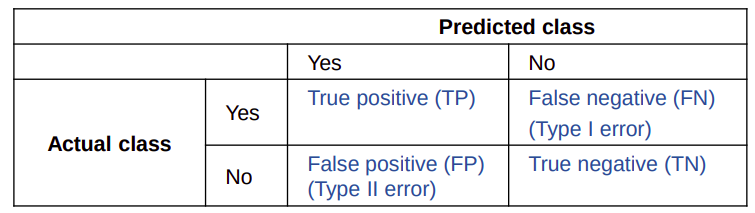
\includegraphics[width=0.65\textwidth]{confusion.png}
\end{figure}
\textbf{Overall Diagonally}:
\subparagraph{Accuracy} $$\text{Accuracy} = \frac{TP + TN}{N}$$
\subparagraph{Error Rate} $$\text{Error Rate} = 1 - \text{Accuracy} = \frac{FP + FN}{N}$$

\textbf{Specific Horizontally}:
\subparagraph{True Positive Rate / Recall / Hit Rate} $$\text{True Positive Rate/Recall} = \frac{TP}{TP + FN}$$
\subparagraph{True Negative Rate / Specificity} $$\text{True Negative Rate/Specificity} = \frac{TN}{TN + FP}$$
\subparagraph{False Positive Rate / False Alarm Rate} $$\text{False Positive Rate/False Alarm Rate} = 1- \text{Specificity} = \frac{FP}{TN + FP}$$

\textbf{Specific Vertically}:
\subparagraph{Precision} $$\text{Precision} = \frac{TP}{TP + FP}$$


\textbf{Cost-Sensitive Learning}:
\begin{itemize}
	\item Goal of general test data evaluation: minimize \textbf{overall error rate}
	
	$\rightarrow$ same weight on each prediction
	
	\item Idea in cost-sensitive learning: 
	\begin{itemize}
		\item unbalanced data
		\item prediction has different cost
	\end{itemize}
	\item Goal in cost-sensitive learning: minimize \textbf{cost}
	\item Solution:
	\begin{itemize}
		\item \textbf{weighting} of instance according to cost
		\item \textbf{resampling} of instance according to cost
		\item \textbf{predict probabilities} instead of predicting classes. minimize the cost by selecting a better \textbf{cutoff-value} (default: 0.5)
	\end{itemize}
	$\rightarrow$ the model \textbf{biased towards cost-sensitive} prediction. 
	
	$\rightarrow$ eg: in churn prediction, better predict more churns (more false positives as false negatives)
\end{itemize}


\subsubsection{Gain Curve}
\begin{itemize}
	\item Idea: visualize results of \textbf{different cutoffs}.
	
	$\rightarrow$ the \textbf{gain most of the targets} by just taking \textbf{a percentage of the whole dataset}, no need to go through the whole.
	
	$\rightarrow$ evaluate models in \textbf{cost-sensitive learning}
	\item Process:
	\begin{itemize}
		\item predict probabilities instead of classes.
		\item \textbf{sort} instances by probability \textbf{in descending order}	
	\end{itemize}
	\item x-axis: percentage of the dataset 
	\item y-axis: percentage of \textbf{actual true} instances in the whole given dataset
\end{itemize}
\begin{figure}[H]
	\centering
	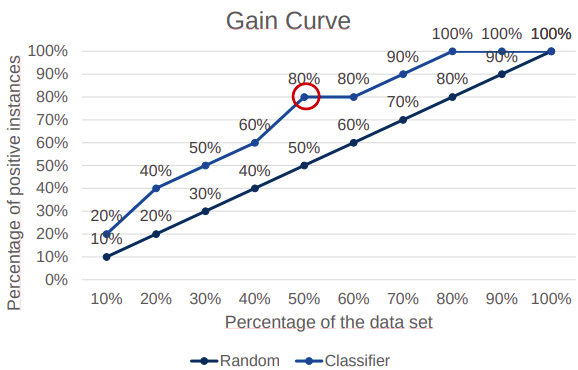
\includegraphics[width=0.55\textwidth]{gain.png}
\end{figure}
\subsubsection{Lift Curve}
\begin{itemize}
	\item Idea: visualize \textbf{how much better} sorting and taking the q\% of data set is than random sampling q\%.
	
	\item x-Axis: percentage of the dataset $q$
	\item y-Axis: Ratio of sorting and taking the q\% to random sampling 
		
	$\rightarrow$ min(Lift) = 1
		
	$$\text{Lift}(q) = \frac{\text{Gain}(q)}{q}$$

\end{itemize}
\begin{figure}[H]
	\centering
	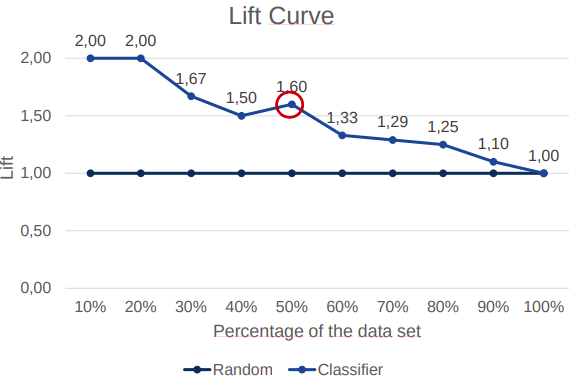
\includegraphics[width=0.55\textwidth]{lift.png}
\end{figure}
\subsubsection{ROC Curve}
\begin{itemize}
	\item Idea: go through all sizes of samples
	\item x-Axis: false positive rate
	\item y-Axis: true positive rate
	\item Process: 
	\begin{itemize}
		\item \textbf{sort} the predicted probability (the given table might be unsorted).
		\item increase the sample size \textbf{step-wise} as a cutoff for positive prediction, 
		\begin{itemize}
			\item with one more true positive (+), \textbf{go up} one step.
			\item with one more false positive(-), \textbf{go right} one step
		\end{itemize}
		 
	\end{itemize}
	\item Choosing cut-off value: choose the \textbf{percentage that bends to the left the most}.
	\item Comparing 2 models: choose the model that \textbf{bends to the left} the most.
	\item Mark the cut-off value: find the corresponding \textbf{instance predicted at cut-off value}.
\end{itemize}
\begin{figure}[H]
	\centering
	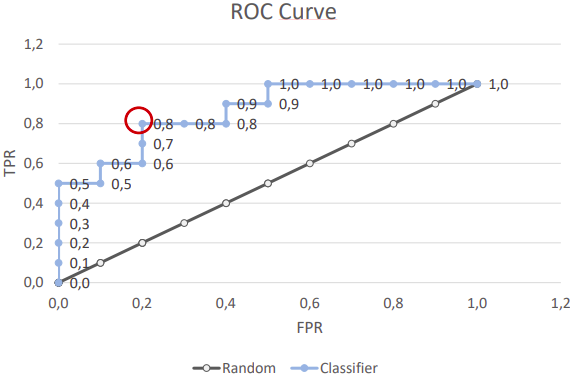
\includegraphics[width=0.55\textwidth]{roc.png}
\end{figure} 

	\section{Dimensionality Reduction}
\begin{itemize}
	\item Reasons: 
	\begin{itemize}
		\item reduce a complex dataset to a \textbf{lower dimension}.
		\item simplify data understanding, visualization and manipulation
		\item reduce computation time
		\item reveal hidden dynamics -- latent variables, \textbf{multicollinearity}
		\item the data lies on a lower dimensional subspace anyway. 
	\end{itemize}

	\item Techniques to Dimensionality Reduction (combat multicollinearity):
	\begin{itemize}
		\item Subset Selection 
		\begin{itemize}
			\item Best Subset, Forward Selection, Backward Elimination, Stepwise Selection
		\end{itemize}
		\item Derived Input in Regression
		\begin{itemize}
			\item Principal Component Regression
			\item Partial Least Squares
		\end{itemize}
		\item Regularization (Coefficient Shrinkage)
		\begin{itemize}
			\item Subset selection
			\item Ridge Regression
			\item Lasso Coefficient
		\end{itemize}
	\end{itemize}
	
	\item Comparison Linear Regression VS. Dimension-Reduction Techniques
	\begin{itemize}
		\item Linear Regresion: 
		\begin{itemize}
			\item requires $n \geq p$, more observations than variables. 
			
			$\rightarrow$ reality large observation too costly, variables too much
			\item if number of variables too large $\rightarrow$ \textbf{Overfitting}
			\item can't combat multicollinearity, separate test on VIF.
			\item \textbf{unstable} to little variability on data in prediction results
		\end{itemize}
		\item Dimension-Reduction Techniques:
		\begin{itemize}
			\item PCR: combats multicollinearity through computing linear uncorrelated principal components.
			\item \textbf{more stable} to the variability on data if variables are correlated.
			\item Regularization: through feature selection, introduce \textbf{bias} but \textbf{reduce variance (smaller MSE)}.  
		\end{itemize}
	\end{itemize}
\end{itemize}
\subsection{Principal Component Analysis}
\begin{itemize}
	\item Definition: converts a set of possibly \textbf{correlated} variables into a (possibly smaller) set of \textbf{linearly uncorrelated} variables -- \textbf{Principal Components}.
	
	\item Goal: transform the data, such that the new dimensions are \textbf{linear uncorrelated} and we \textbf{maximize the variance} along the axes.
	\item Assumption: relationship among variables is \textbf{linear}.
	\item \textbf{Principal Components}: \textbf{explain most of the variability} in the original dataset. 
	\begin{itemize}
		\item the \textbf{eigenvectors} of the covariance/correlation matrix
		\item the direction are those in feature space along which the original data is \textbf{highly variable}.
		\item the \textbf{first PC} has \textbf{largest possible variance}.  It's the direction of \textbf{maximum variance from origin}.
		\item \textbf{subsequent PCs} are \textbf{orthogonal} to first PC. They describe \textbf{maximum residual variance}.
		\item each element of eigenvector represents the \textbf{contribution of a variable} to the PC.
	\end{itemize}
	\item PCA \textbf{Eigenvalues}: give the \textbf{proportion of variance explained} by the corresponding principal components. 
	\begin{itemize}
		\item $\lambda_1$ shows the proportion of variance explained by PC1. $\rightarrow$ the \textbf{spread of data} in PC1 direction.
	\end{itemize}
	\item PCA \textbf{Scores}: Z, score of x are the coefficients of in each PC direction. 
\end{itemize}

\subsubsection{Process}
\begin{enumerate}[label= \protect \circled{\arabic*} ]
	\item \textbf{center} the data, subtract the \textbf{mean} from each data dimension. $\rightarrow$ zero-mean dataset.
	\item compute \textbf{covariance/correlation matrix}:
	\begin{itemize}
		\item covariance matrix: variables in \textbf{comparable units}, \textbf{difference in variance} across variable \textbf{important}
		\item correlation matrix: variables in \textbf{different units}, \textbf{difference in variance} across variable \textbf{not important}
	\end{itemize}
	$$Var(x_j) =  \frac{1}{N-1} \cdot\Sigma x_{ij}^2$$
	$$Cov(x_{j1}, x_{j2}) = \frac{1}{N-1} \cdot \Sigma x_{ij1} x_{ij2} $$
	
	\item compute \textbf{eigenvalues and eigenvectors} of the covariance/correlation matrix. \textbf{Normalized} the eigenvectors.
	\item \textbf{order} eigenvectors according to \textbf{its eigenvalues in descending order} $\Phi$.
	\item compute variance explained by each principal component:
	$$\text{variance explained} = \frac{\lambda_i}{\Sigma \lambda_i}$$
	\item Project the transformed data onto principal components: all principal components are \textbf{orthonormal basis}.
	$$Z = X\cdot \Phi$$
	\item Compress: choose $k$ most important PCs. $\rightarrow$ slight \textbf{information loss}
\end{enumerate}

\subsubsection{Reconstruction of Original Data}
$$D \approx Z \Phi^T + \text{means}$$

If \textbf{dimensionality reduced}, we \textbf{lose} those dimensions we choose to \textbf{discard}. The information loss is relatively small.
\subsubsection{Computation Principal Component: Singular Value Decomposition}
$$A = U\cdot S \cdot T^{T}$$

\begin{itemize}
	\item Alternative to compute principal components.
	\item principal axes/components: columns of V
	\item principal component scores $U\cdot S$
	\item Use-case: recommendation system
\end{itemize}
\subsection{Principal Component Regression}
\begin{itemize}
	\item Multiple Linear Regression VS. Principal Component Regression
	\begin{itemize}
		\item PC combines the correlated variables into linear uncorrelated variables. It explain the most important variability of the model. 
		
		$\rightarrow$ \textbf{combats multicollinearity and unstability} to minor change in data from linear regression models. 
	\end{itemize}
	\item PCR Model:
	$$y = Z \cdot \gamma + \varepsilon,  \quad \text{with} \quad Z = X \cdot \Phi  $$
	\begin{itemize}
		\item independent variables: principal components in Z
	\end{itemize}
	\item works well when the first few principal components are sufficient to explain most of the variation.
	\item not a feature selection method.
\end{itemize}

\subsubsection{Partial Least Squares}
\begin{itemize}
	\item identifies new features in a \textbf{supervised} way:
	\begin{itemize}
		\item new features \textbf{approximate old features} and are \textbf{related to response}.
		\item weights reflect the covariance structure between \textbf{predictors and response}
	\end{itemize}
	\item requires more complicated iterative algorithms
\end{itemize}

\subsection{Regularization: Ridge Regression}
\subsubsection{Regularization}
\begin{itemize}
	\item Goal: \textbf{introduce bias} into regression solution that can \textbf{reduce variance} relative to OLS solution.
	\item Objective function in regularization:
	$$J(\theta) = L(\theta) + \Omega(\theta)$$
	\begin{itemize}
		\item $L(\theta)$ : training loss, describes \textbf{model fit}
		\item $\Omega(\theta)$: regularization, describes \textbf{model complexity} 
	\end{itemize}
\end{itemize}

\subsubsection{Ridge Regression}
\begin{itemize}
	\item Goal: \textbf{minimizes} a \textbf{penalized} RSS
	\item Penality: \textbf{$\mathbf{l_2}$ penality}
	
	$$\hat{\beta}^{ridge} = \arg\min_{\beta} (RSS + \lambda \cdot\Sigma \beta_j^2)$$
	\begin{itemize}
		\item $\lambda \uparrow$ , coefficients $\rightarrow 0$ 
		\item coefficents will never be exactly 0, but nearly 0.
	\end{itemize}
	\item Evaluation: estimates \textbf{more biased} but have \textbf{lower variance} than OLS-Estimator. 
\end{itemize}


\subsection{Regularization: Lasso}
\begin{itemize}
	\item Goal: \textbf{minimizes quantity}
	\item Penality: \textbf{$\mathbf{l_1}$ penality}
	$$\hat{\beta}^{lasso} = \arg\min_{\beta} (RSS + \lambda \cdot \Sigma |\beta_j|)$$
	
	\item Finding tuning parameter $\lambda$ : select a grid of values + cross-validation
	\item Evaluation \& Comparison Ridge Regression:
	\begin{itemize}
		\item has the effect of forcing some coefficients to be \textbf{exactly zero}, when $\lambda$ is large. 
		
		$\rightarrow$ feature selection
		\item produces \textbf{simpler and more interpretable} models involving only \textbf{subset of predictors}
		\item similar behavior to ridge regression: $\lambda \uparrow$, variance $\downarrow$, bias $\uparrow$.
		\item generate \textbf{more accurate predictions}.
	\end{itemize}
\end{itemize}
	
\end{document}
